\chapter{Massresolution}
Figure \ref{fig:massresolution_all} shows the fits to all bins of \Dz\proton mass for the determination of the massresolution.
The whole method and prodecure is described in section \ref{sec:Massresolution}.
\begin{figure}[hptb]
    \centering
	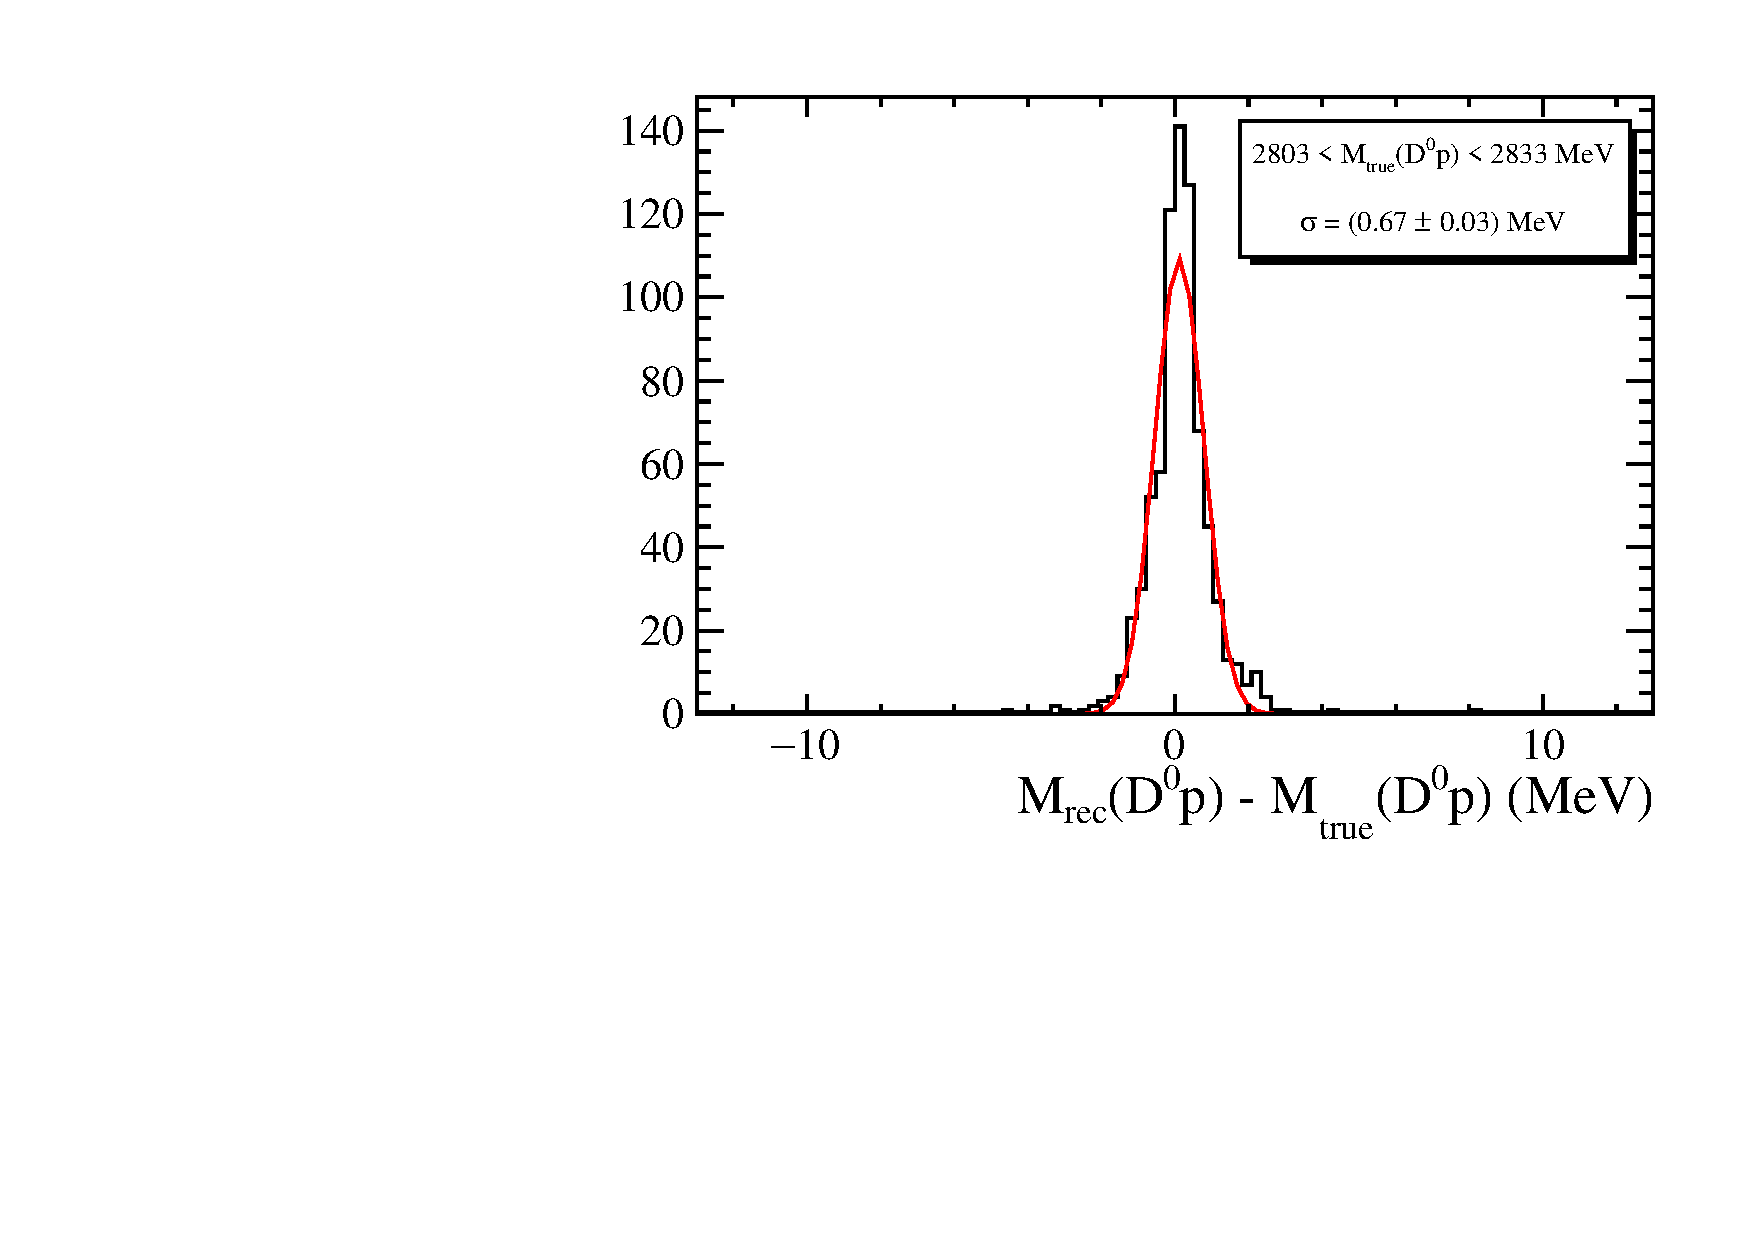
\includegraphics[width=0.32\textwidth]{LbToD0p/massresolution/massresolution_000}
	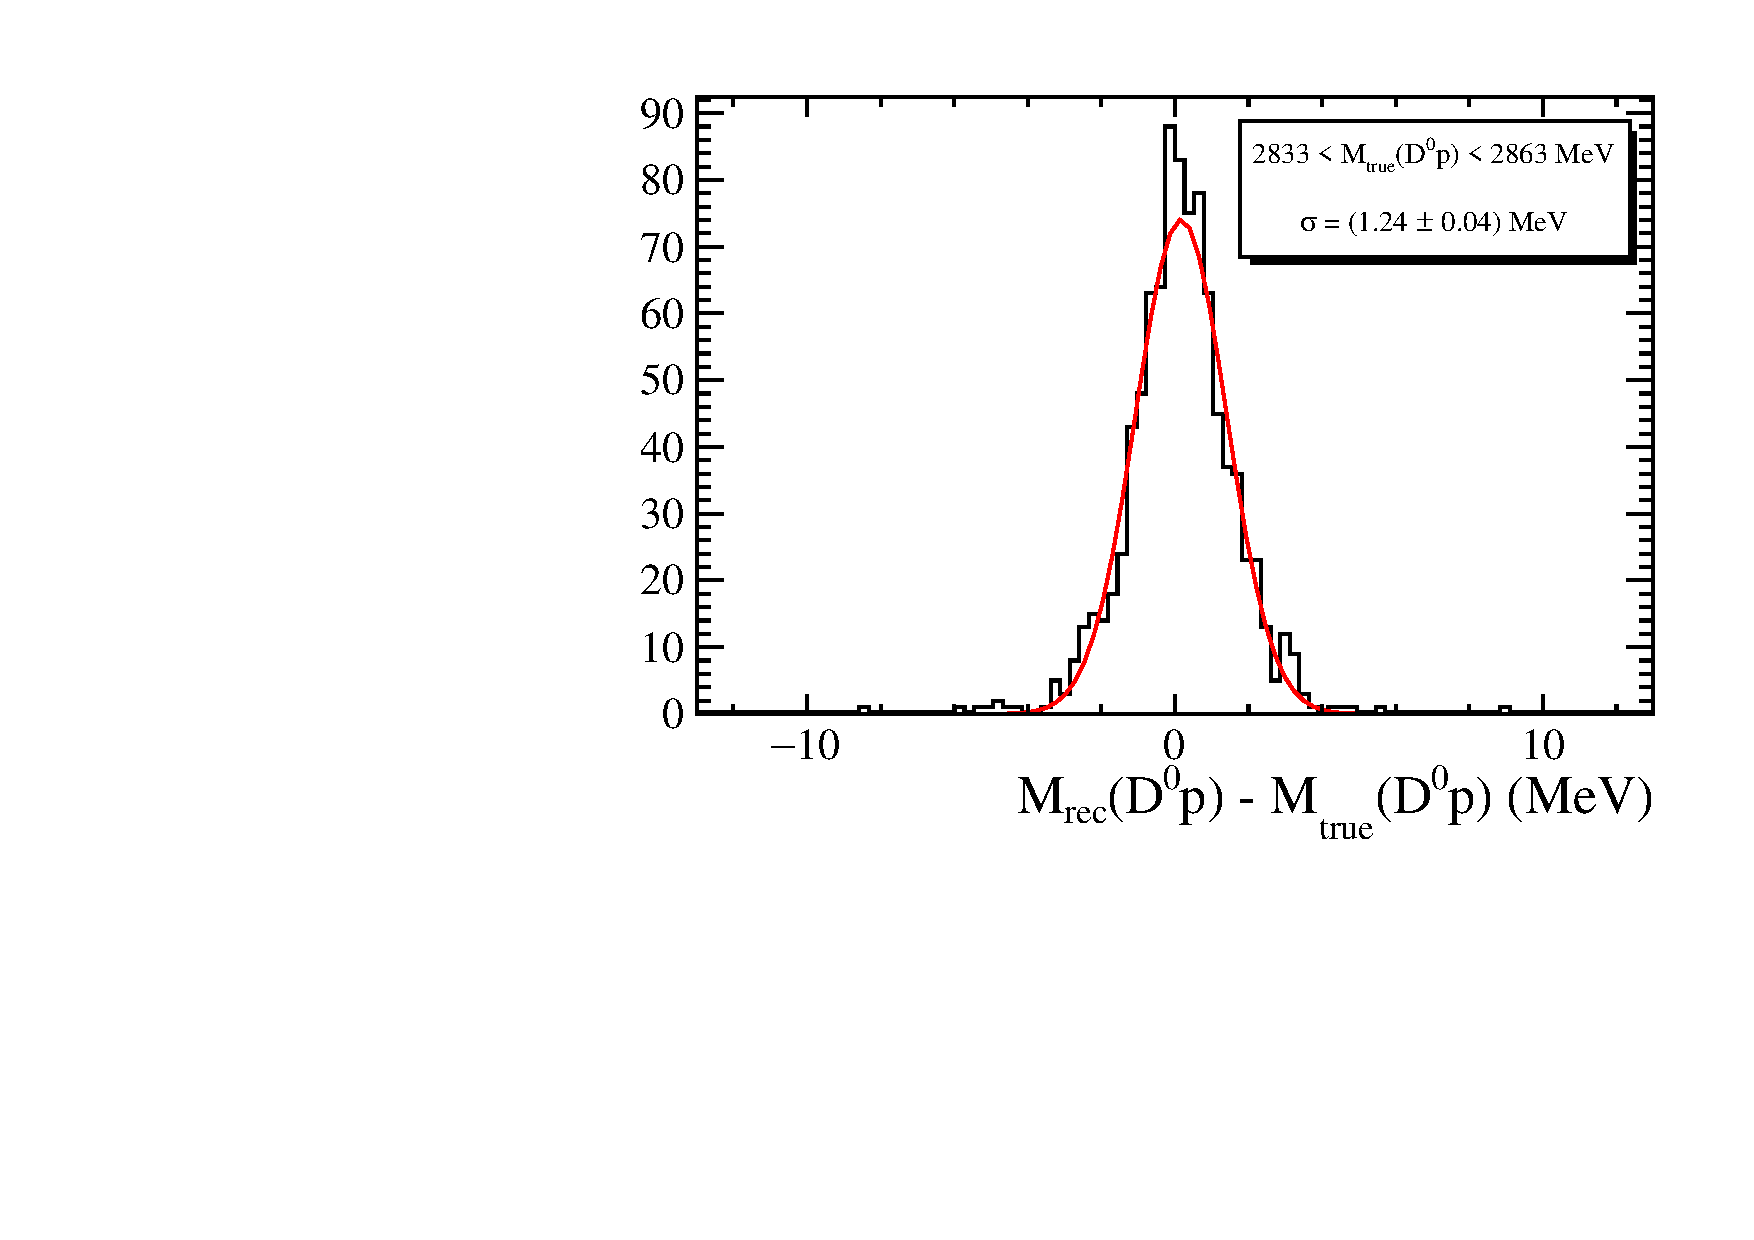
\includegraphics[width=0.32\textwidth]{LbToD0p/massresolution/massresolution_001}
	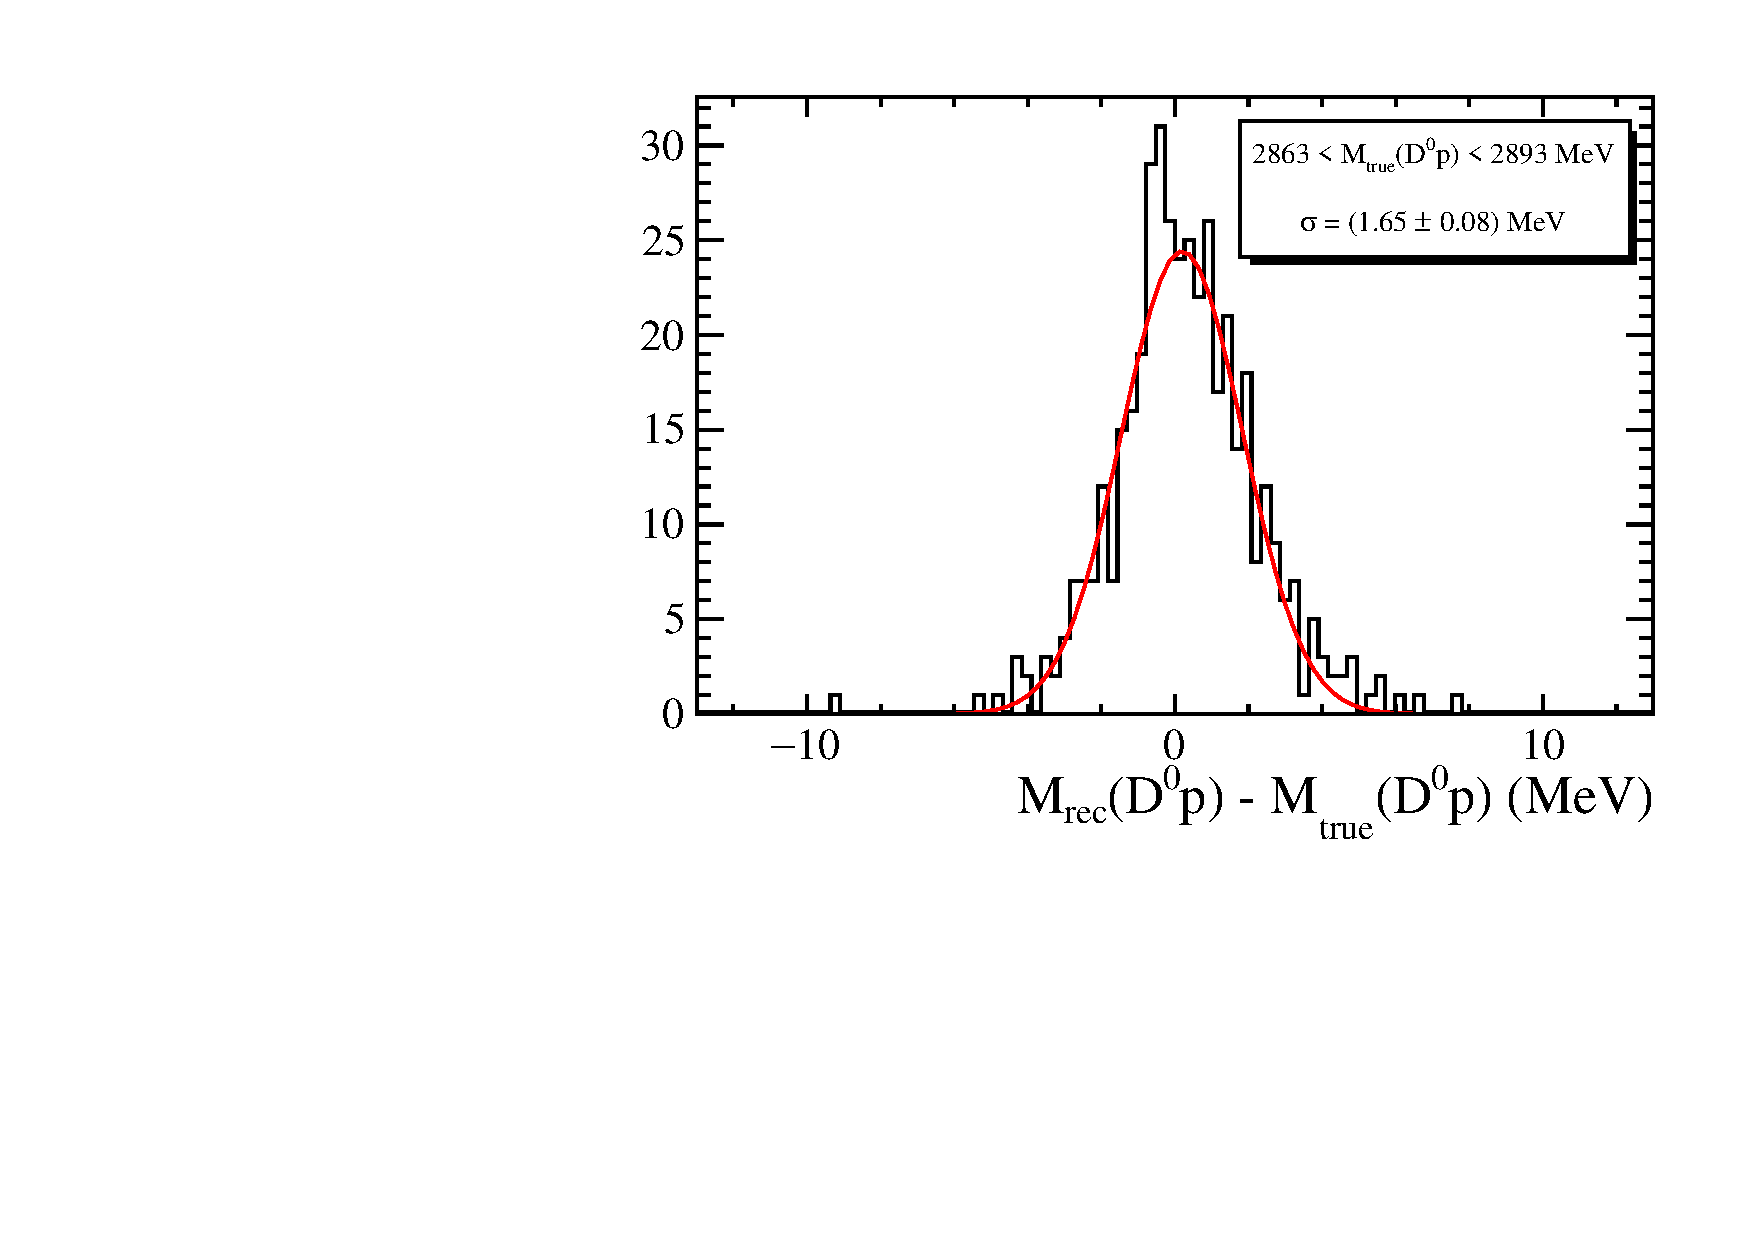
\includegraphics[width=0.32\textwidth]{LbToD0p/massresolution/massresolution_002} \\
	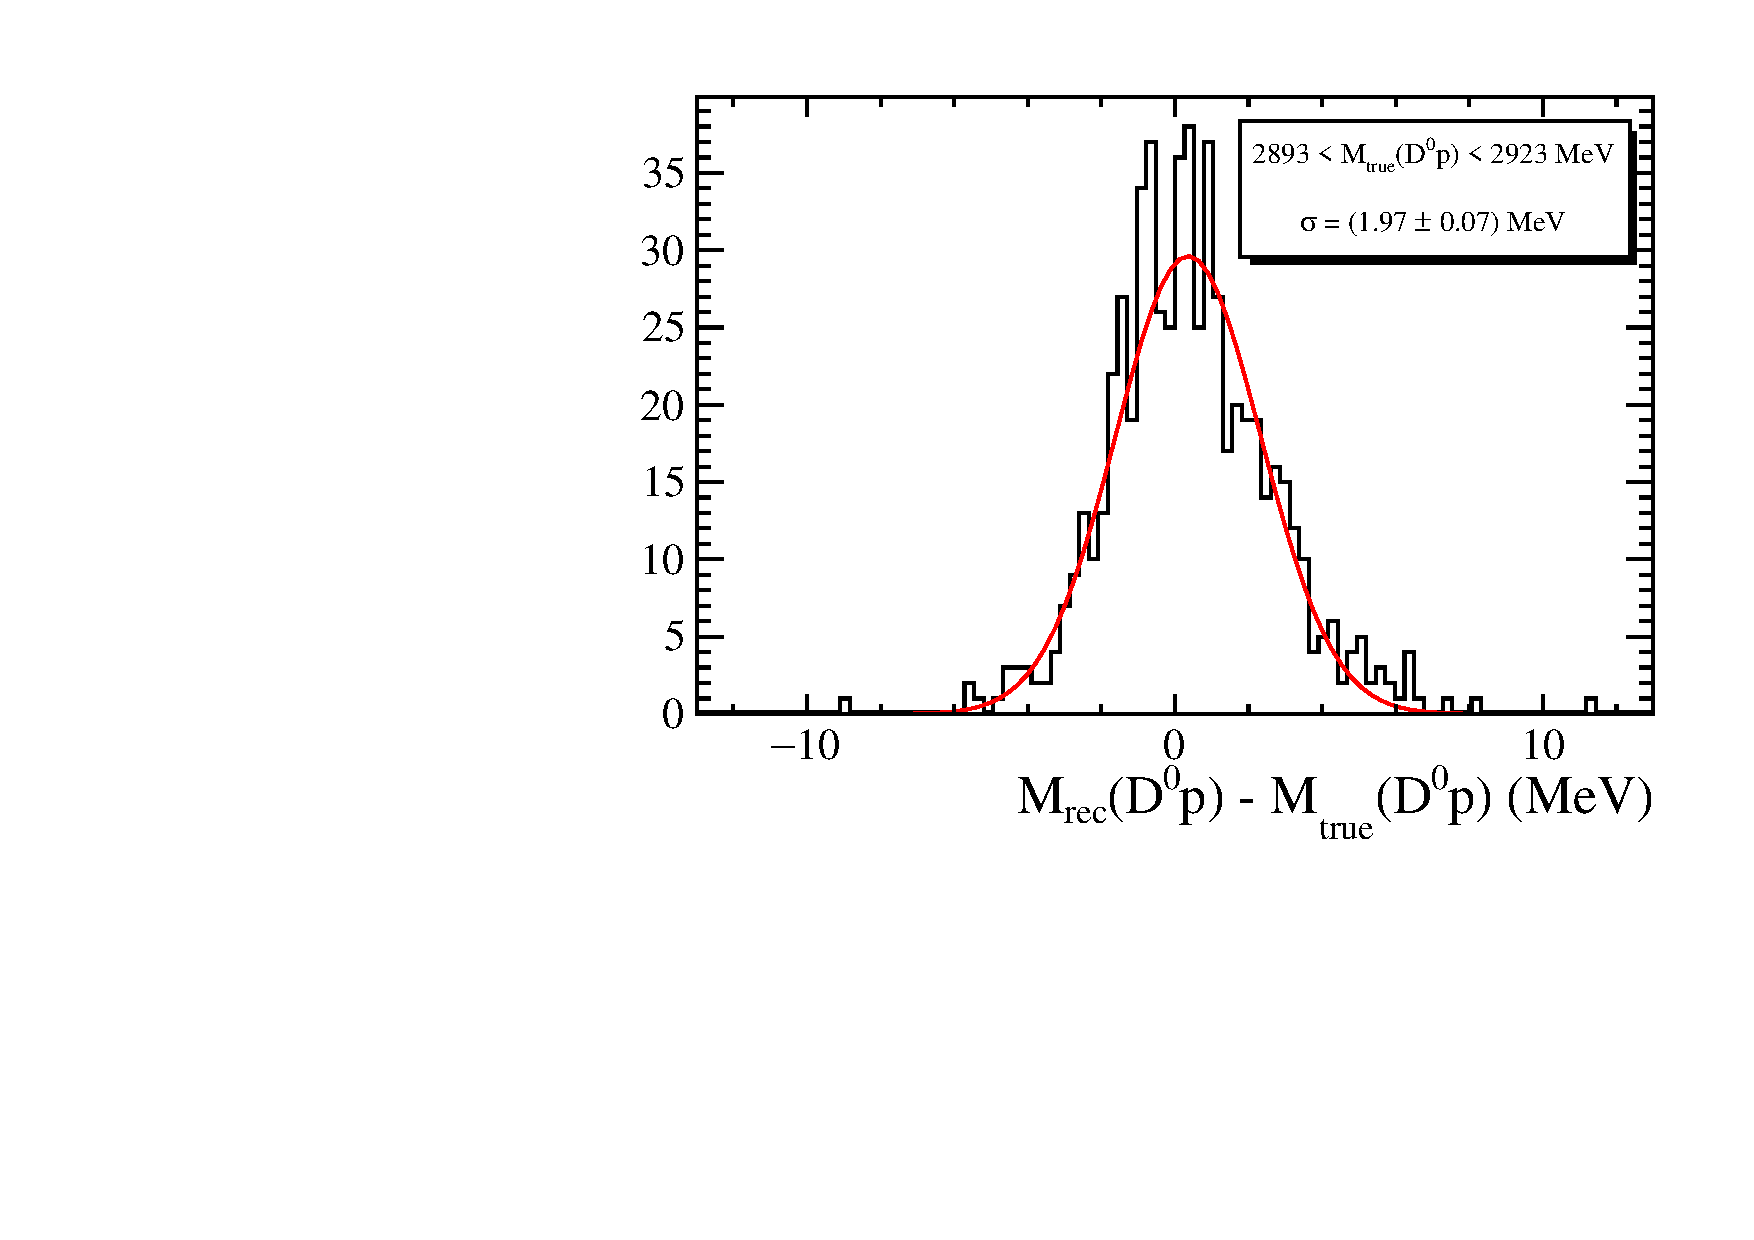
\includegraphics[width=0.32\textwidth]{LbToD0p/massresolution/massresolution_003}
	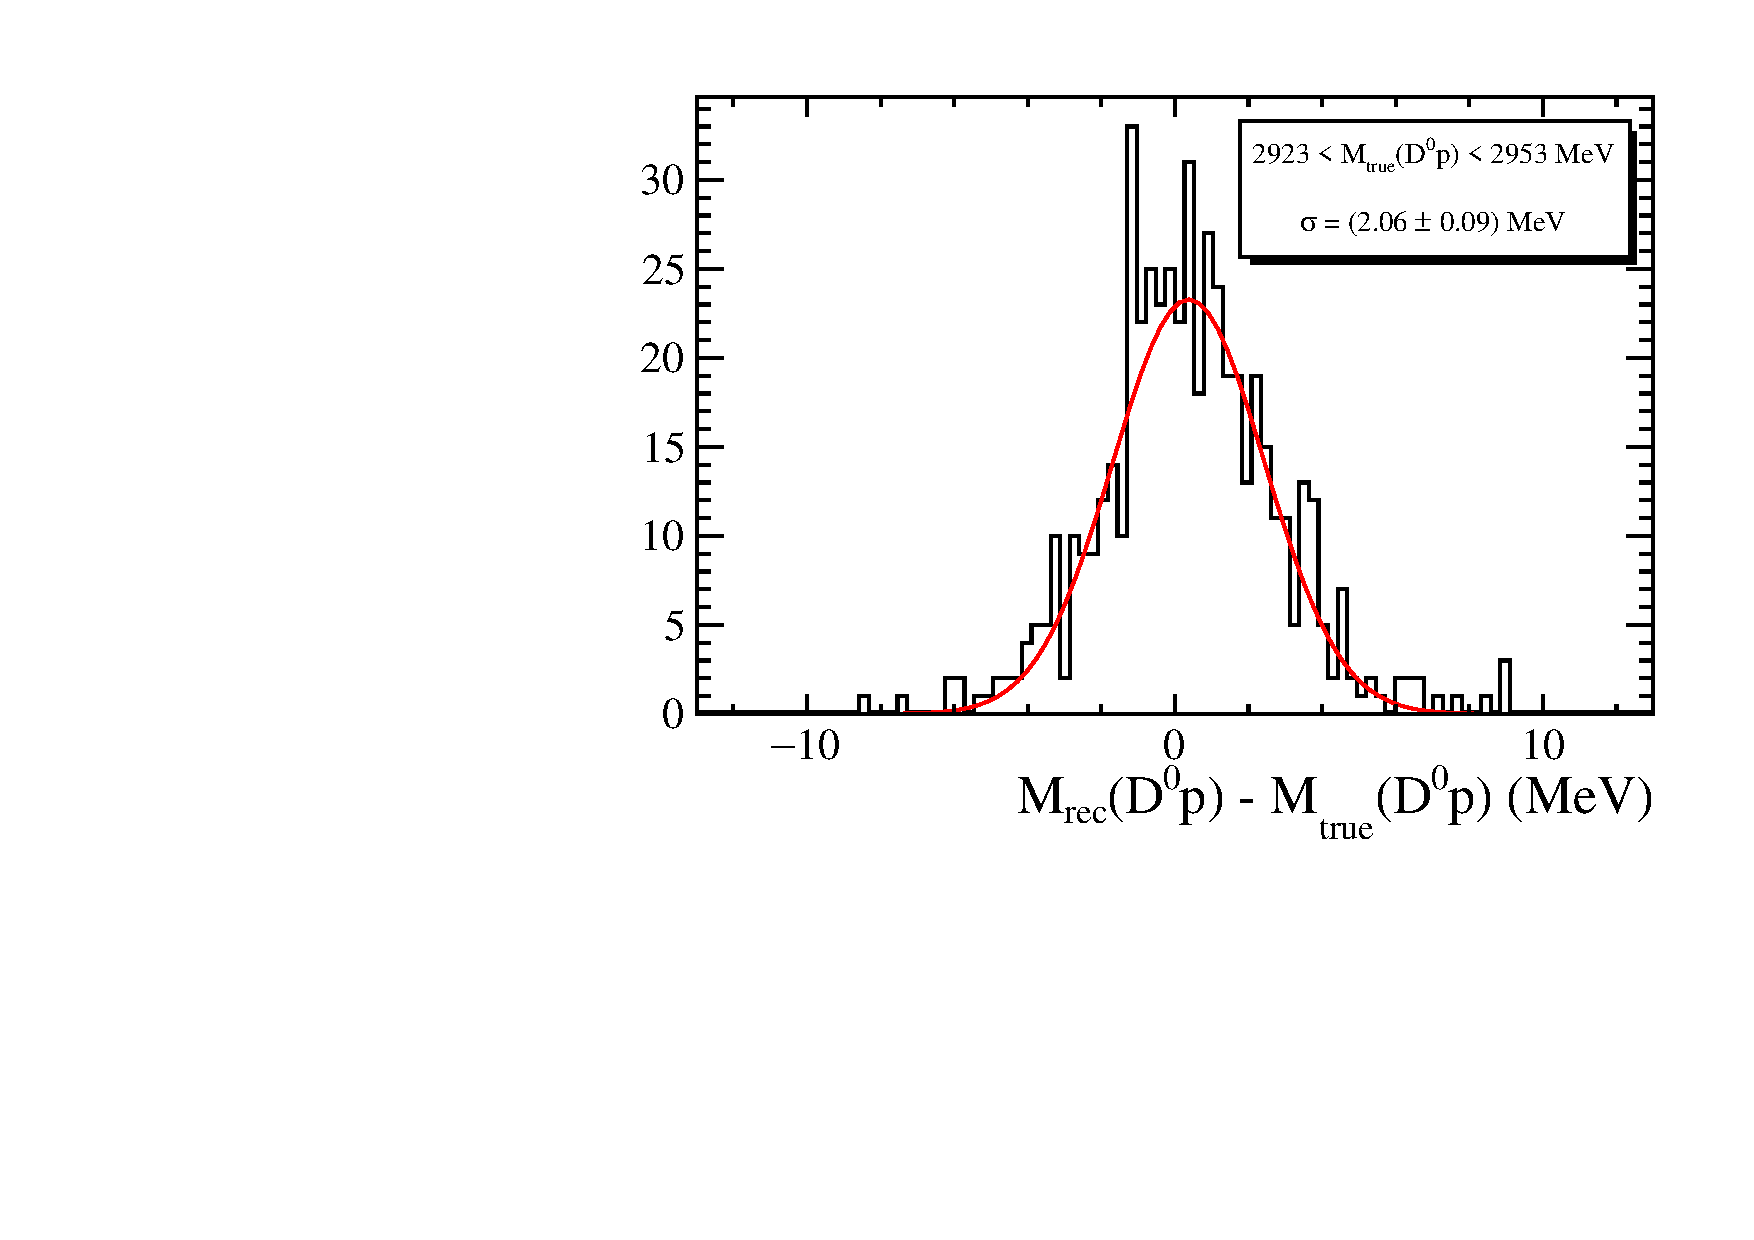
\includegraphics[width=0.32\textwidth]{LbToD0p/massresolution/massresolution_004}
	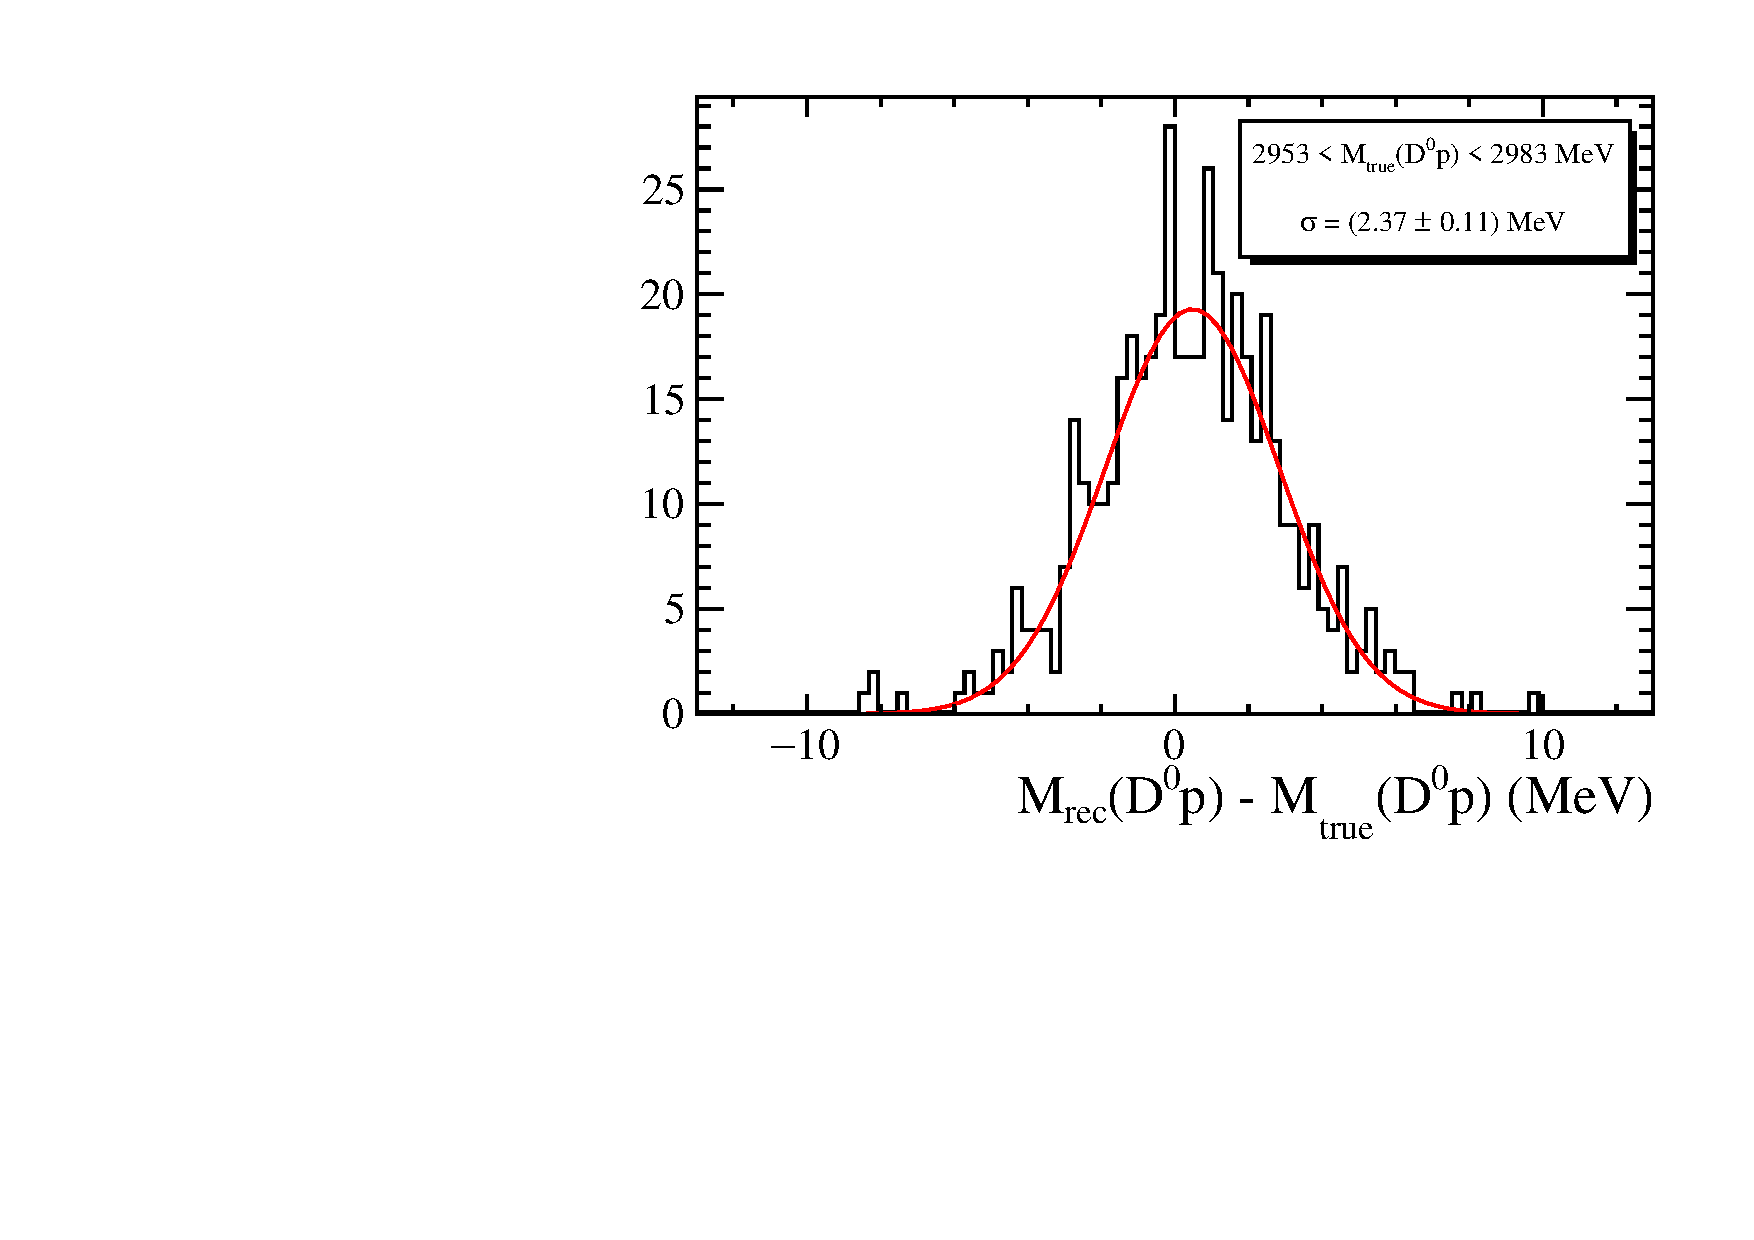
\includegraphics[width=0.32\textwidth]{LbToD0p/massresolution/massresolution_005} \\
	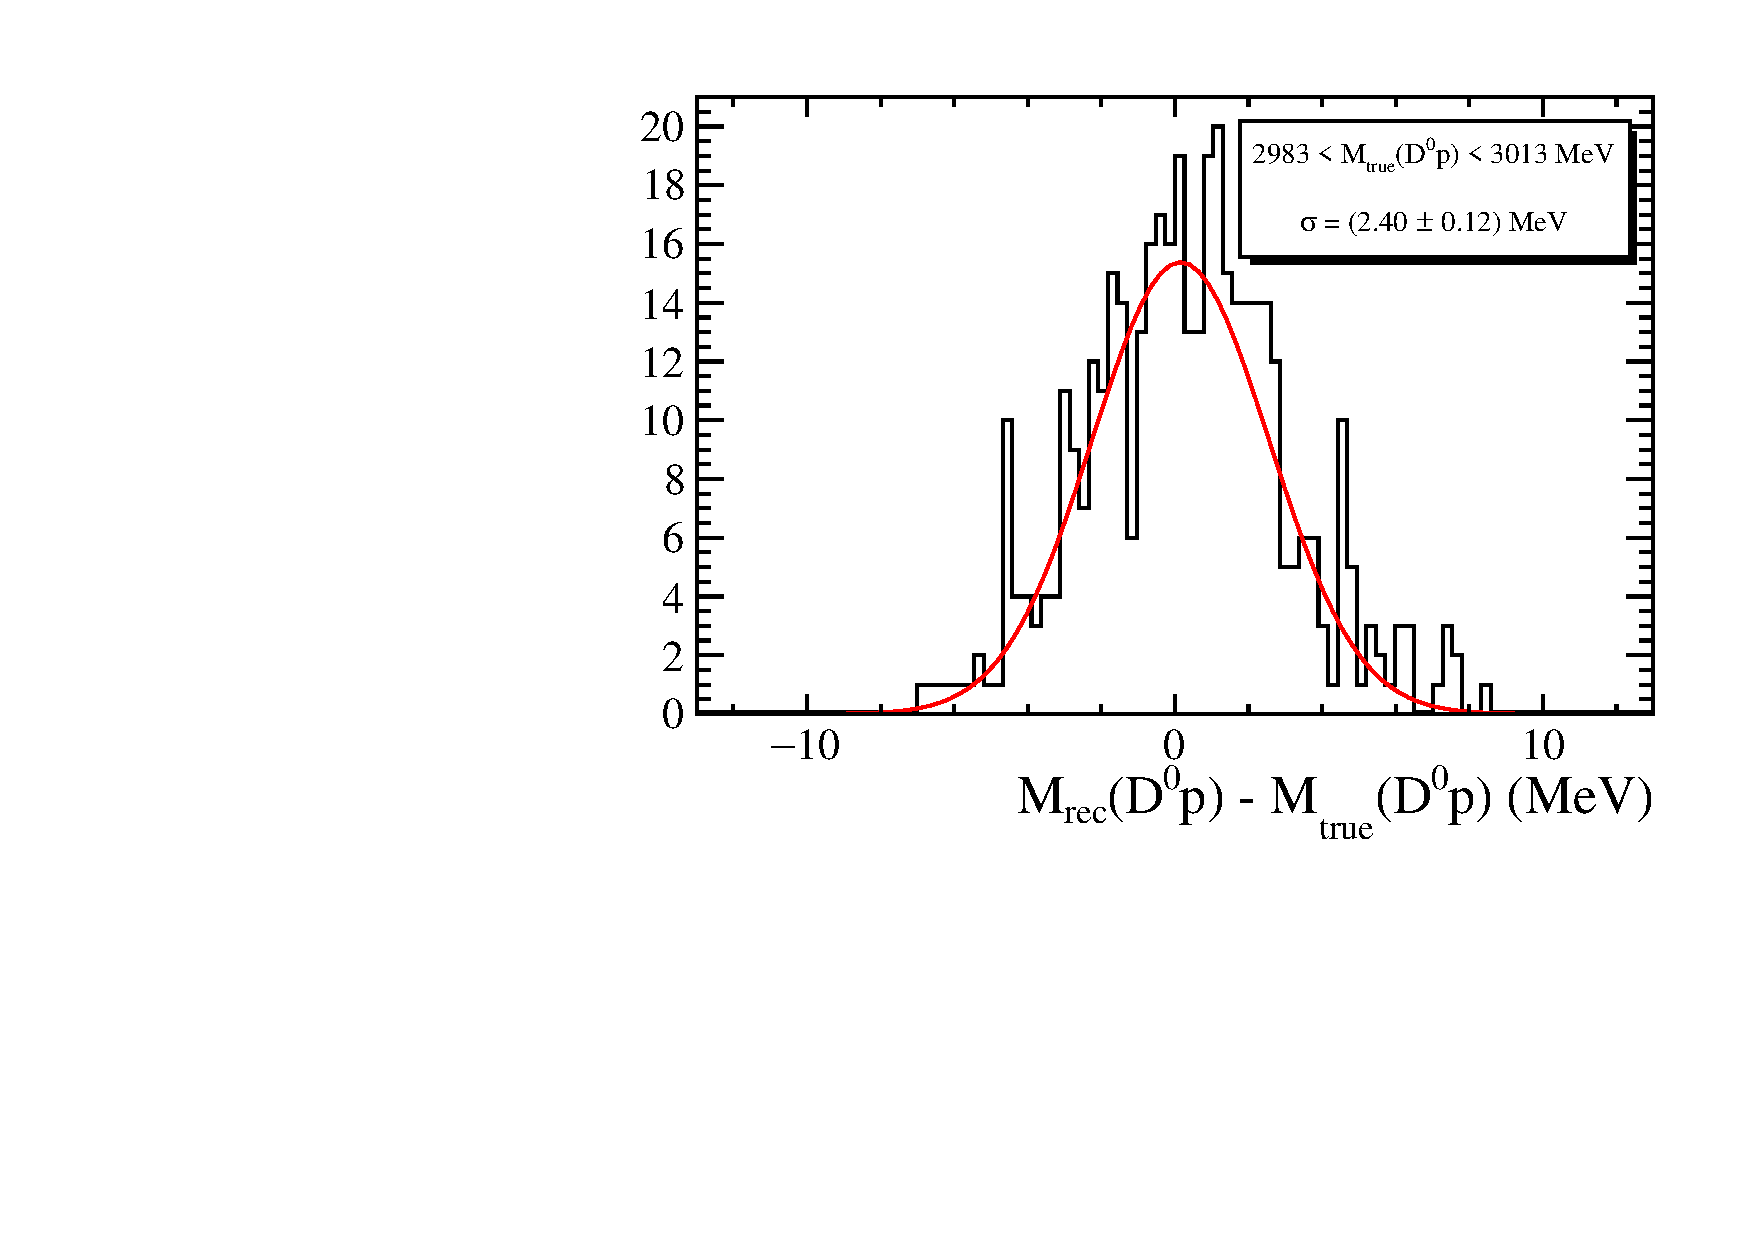
\includegraphics[width=0.32\textwidth]{LbToD0p/massresolution/massresolution_006}
	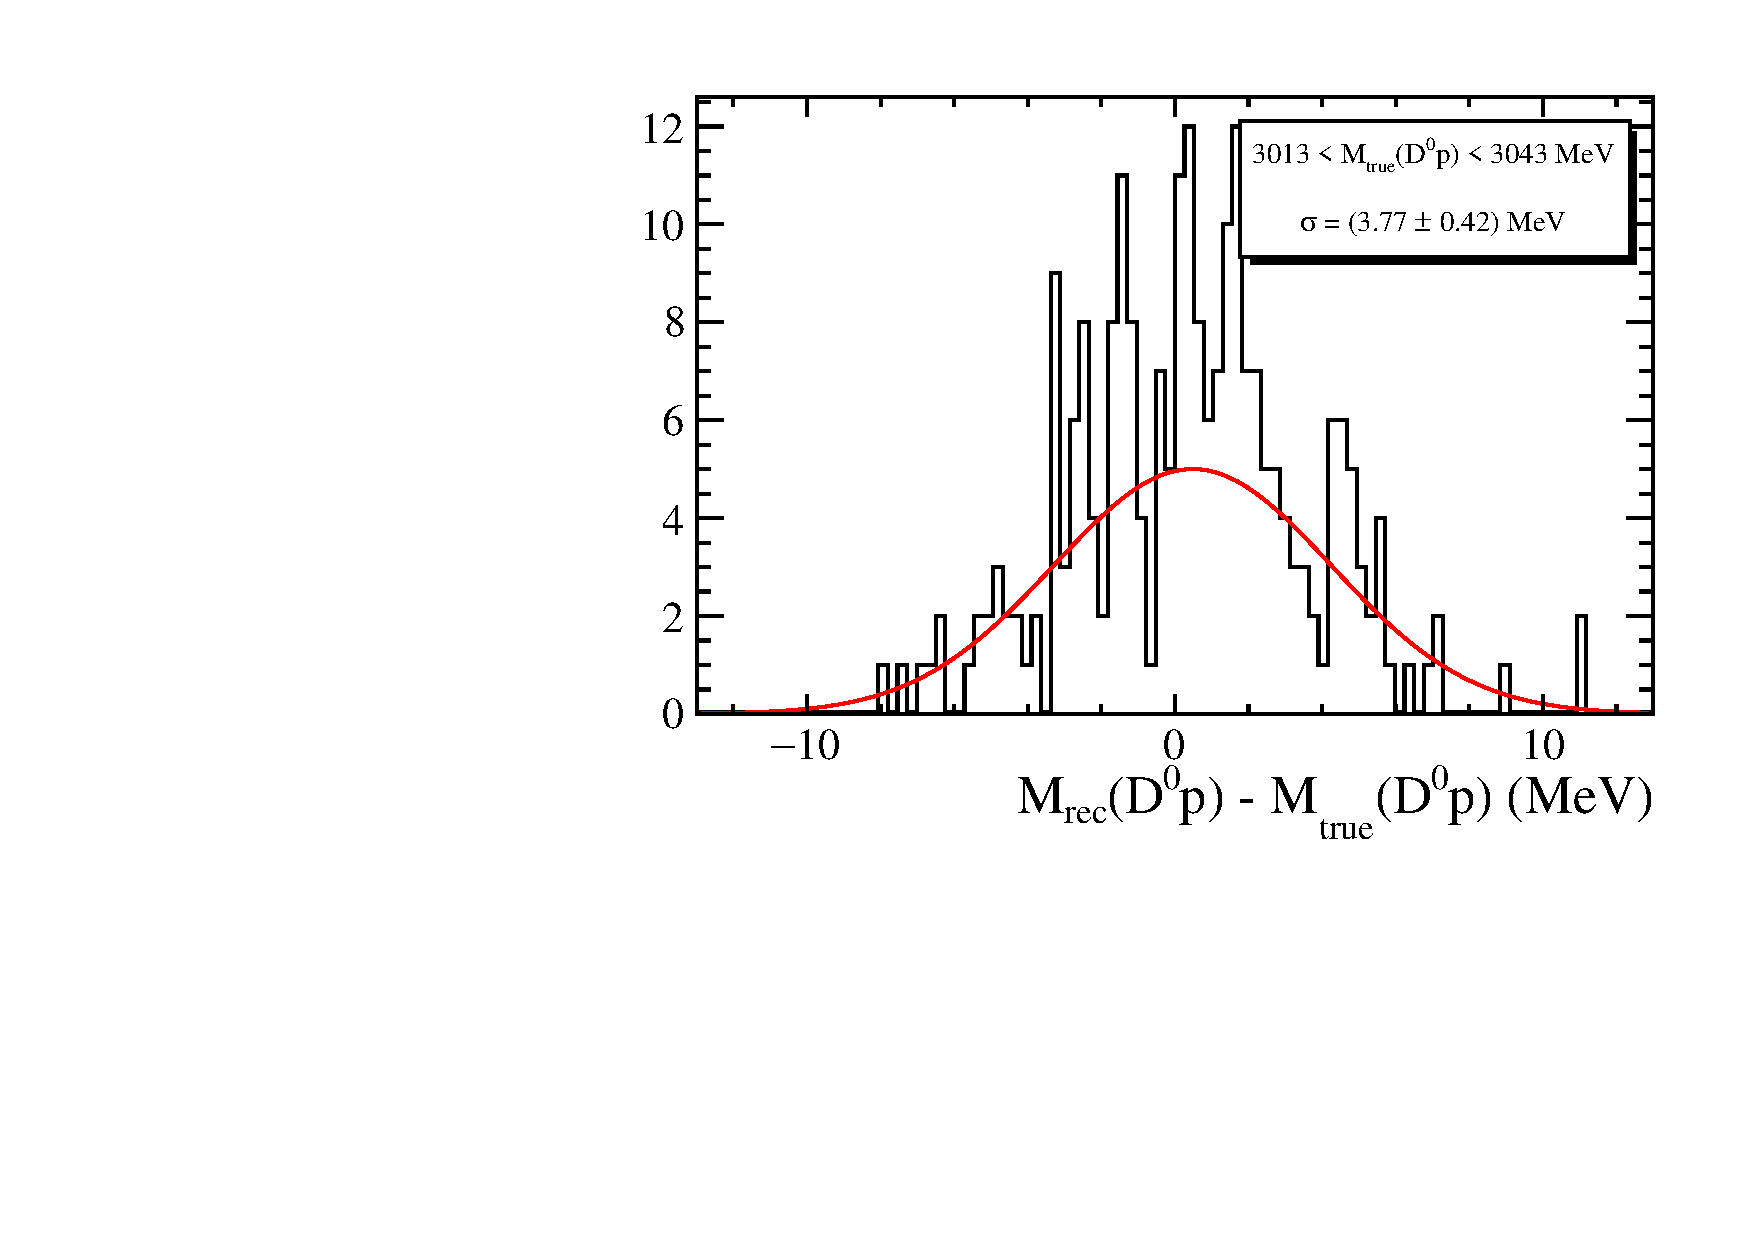
\includegraphics[width=0.32\textwidth]{LbToD0p/massresolution/massresolution_007}
	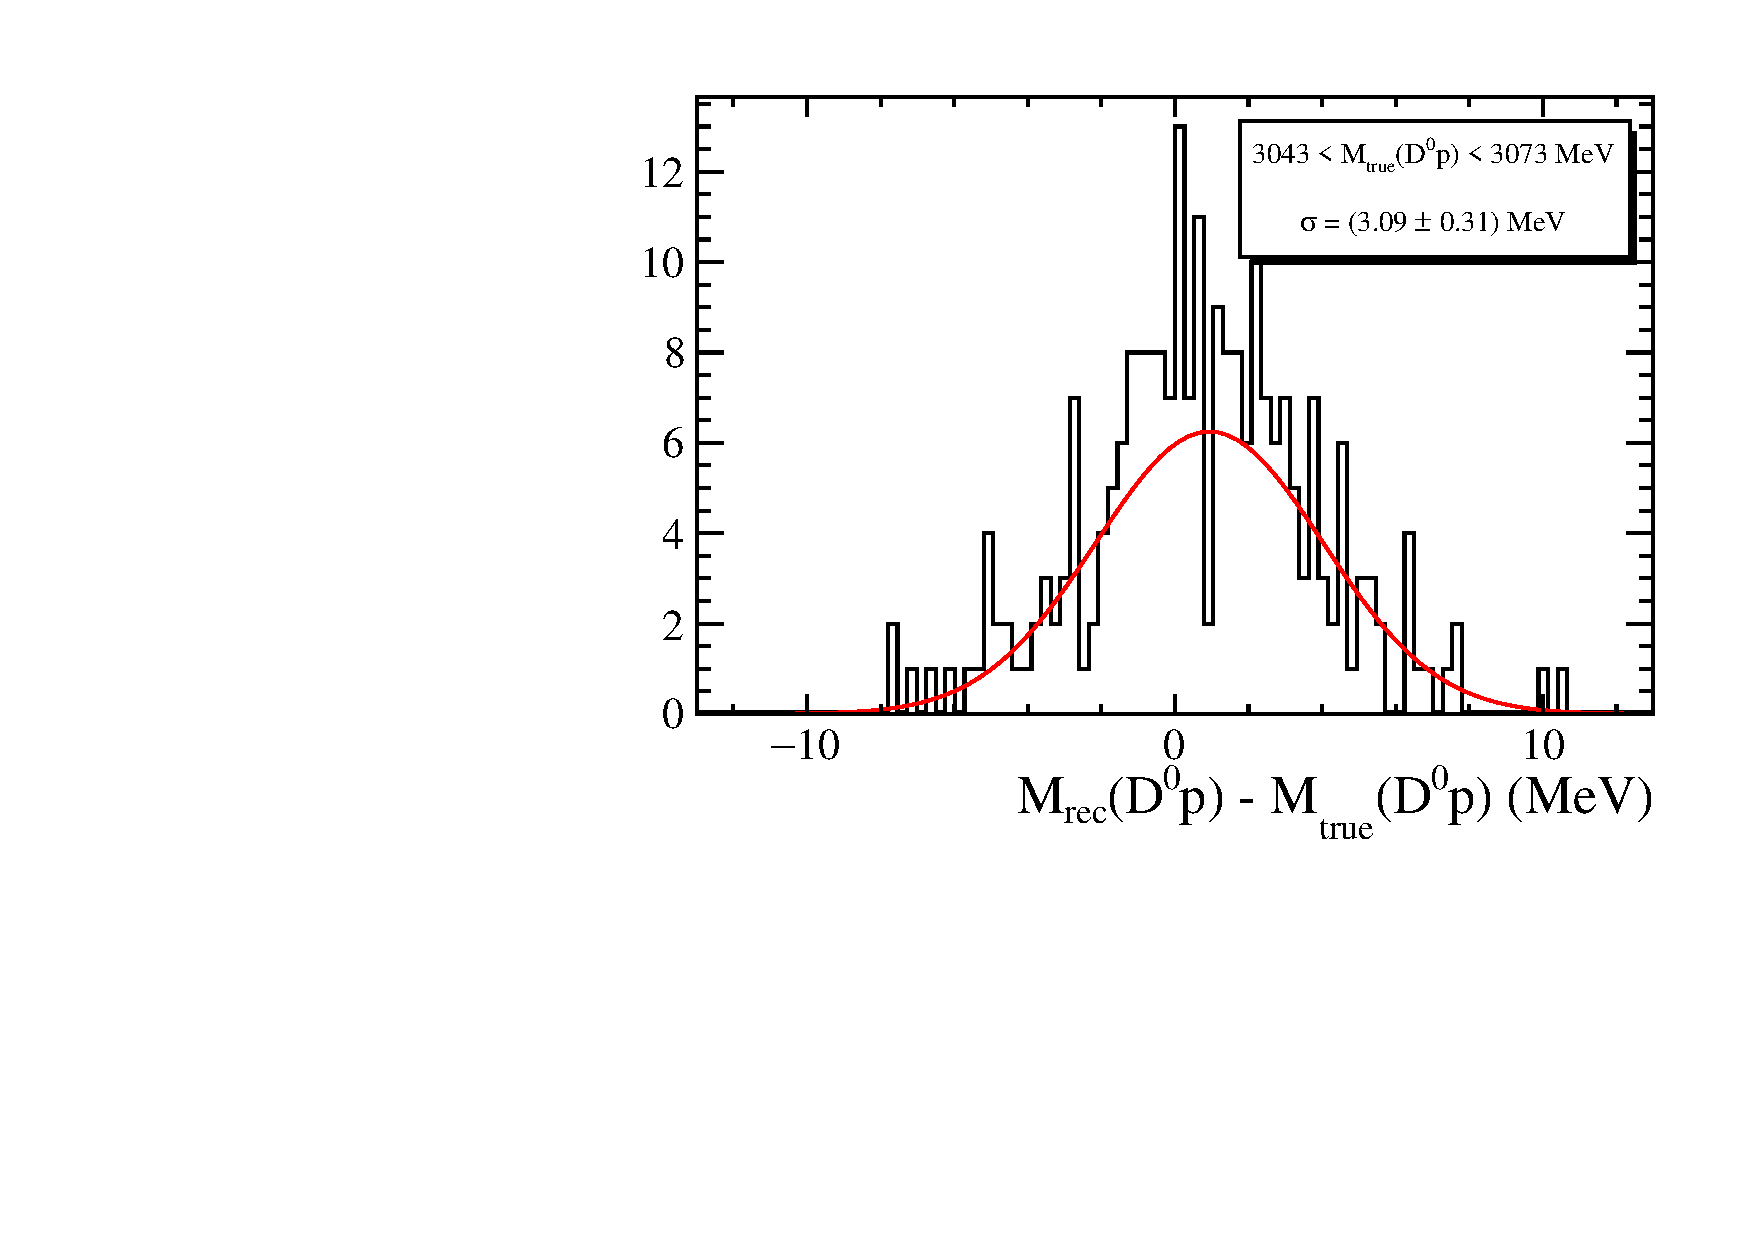
\includegraphics[width=0.32\textwidth]{LbToD0p/massresolution/massresolution_008} \\
	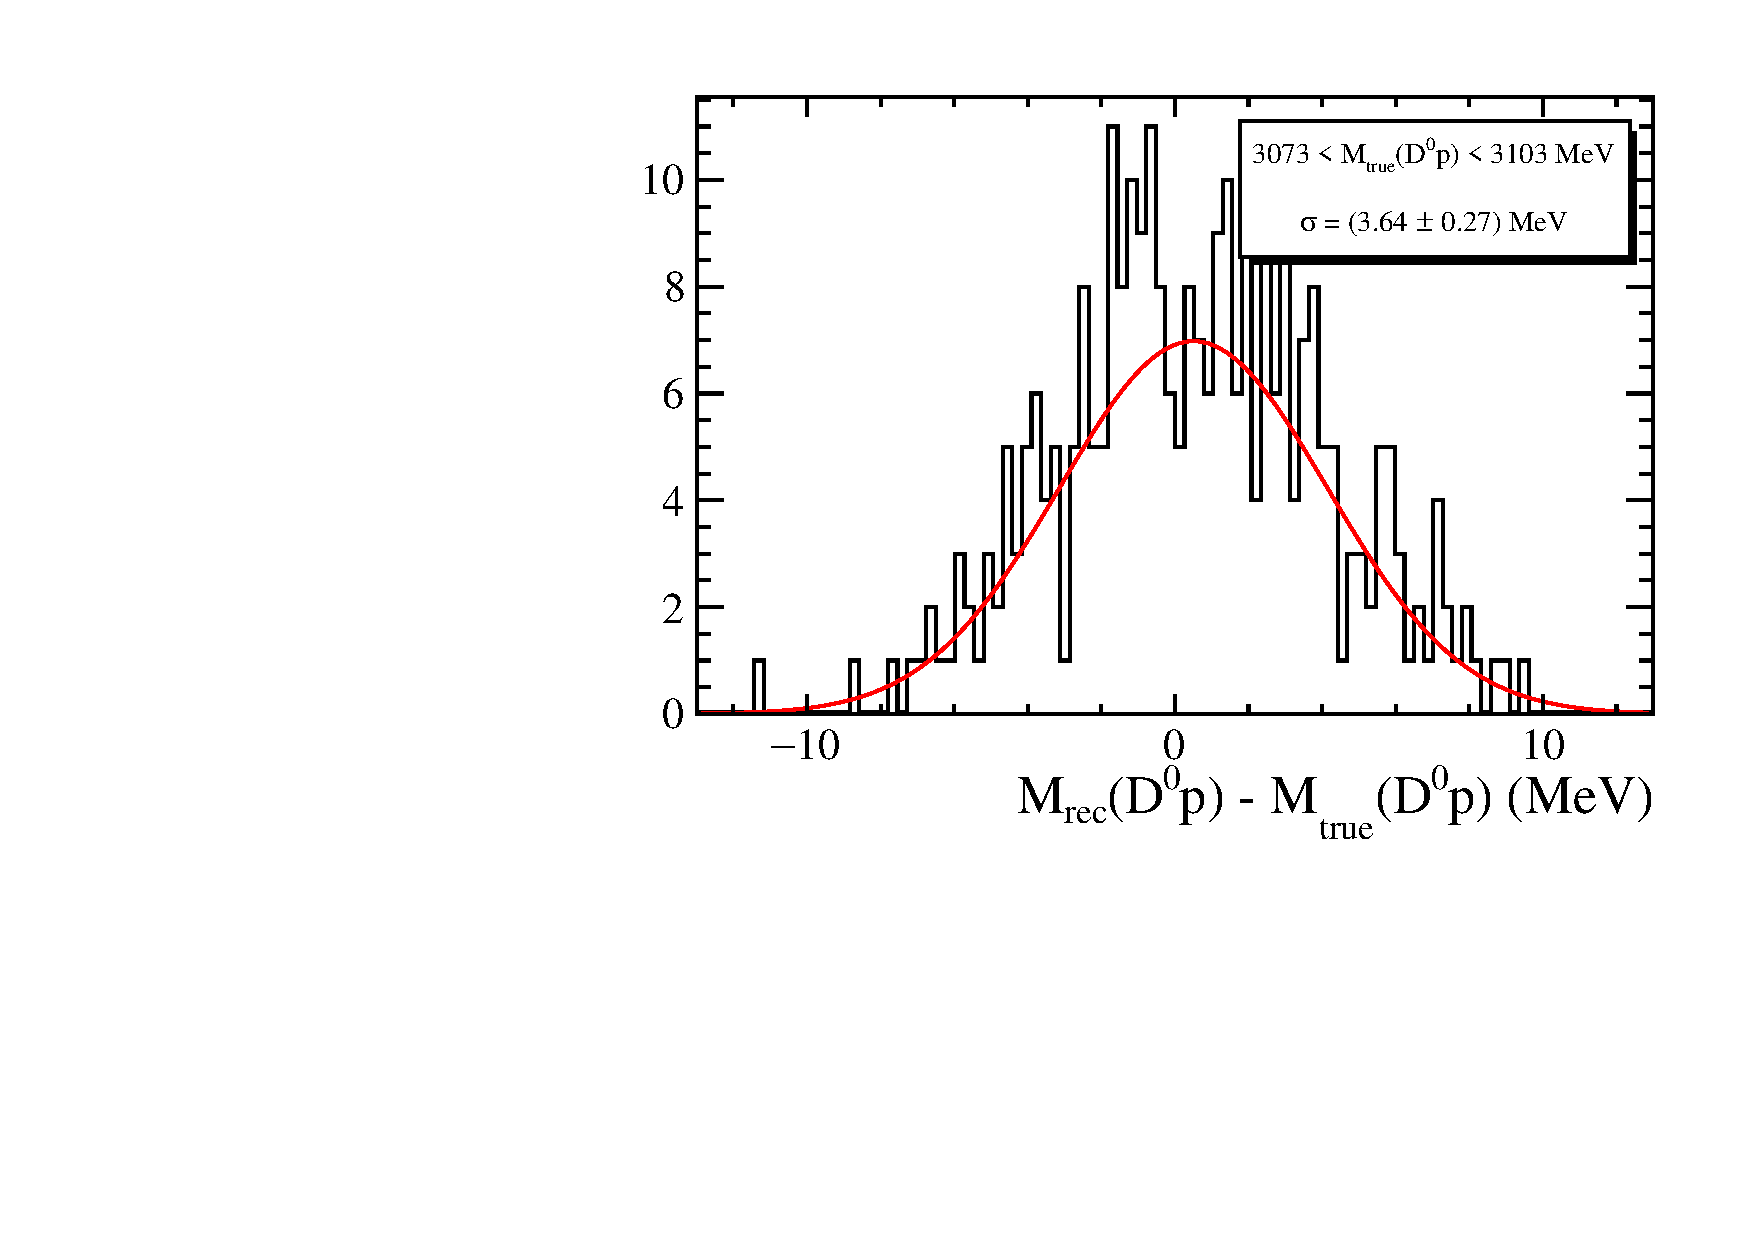
\includegraphics[width=0.32\textwidth]{LbToD0p/massresolution/massresolution_009}
	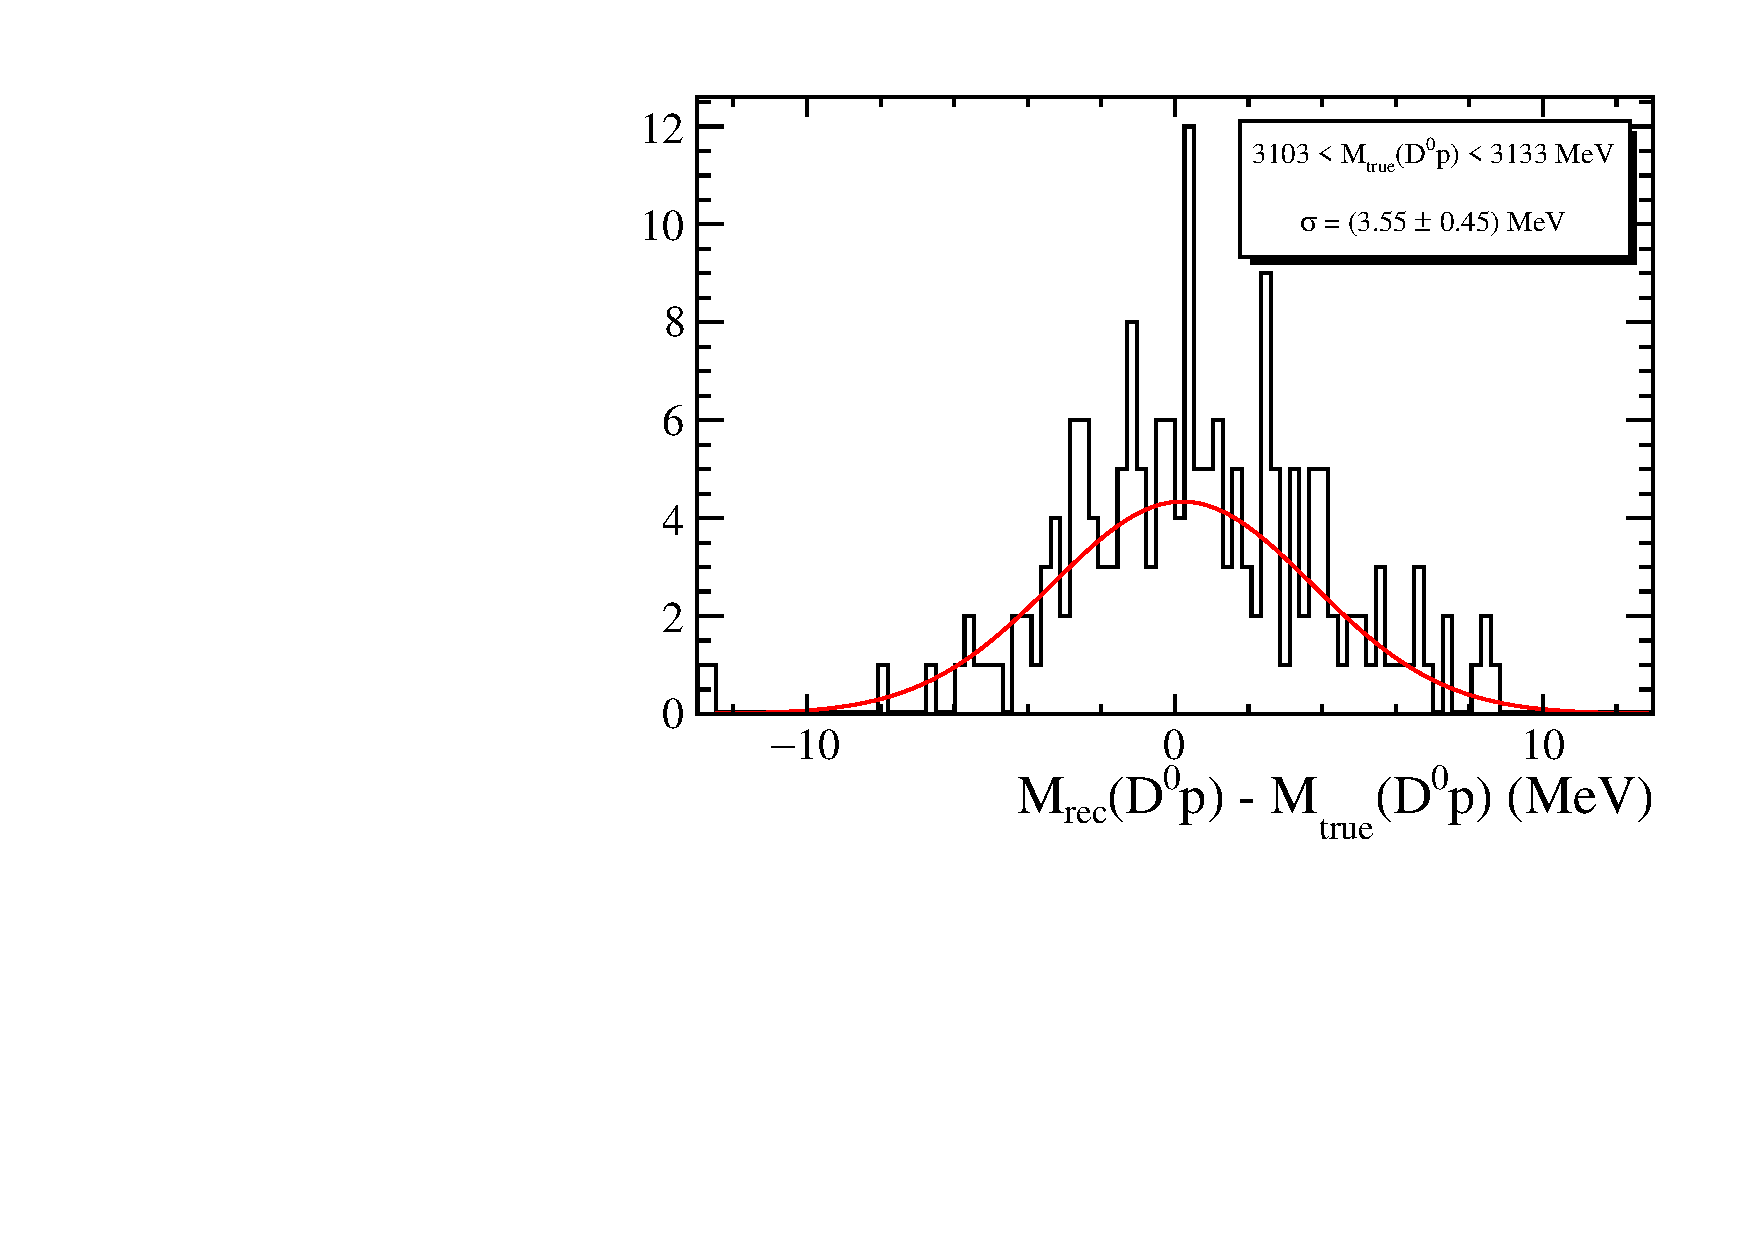
\includegraphics[width=0.32\textwidth]{LbToD0p/massresolution/massresolution_010}
	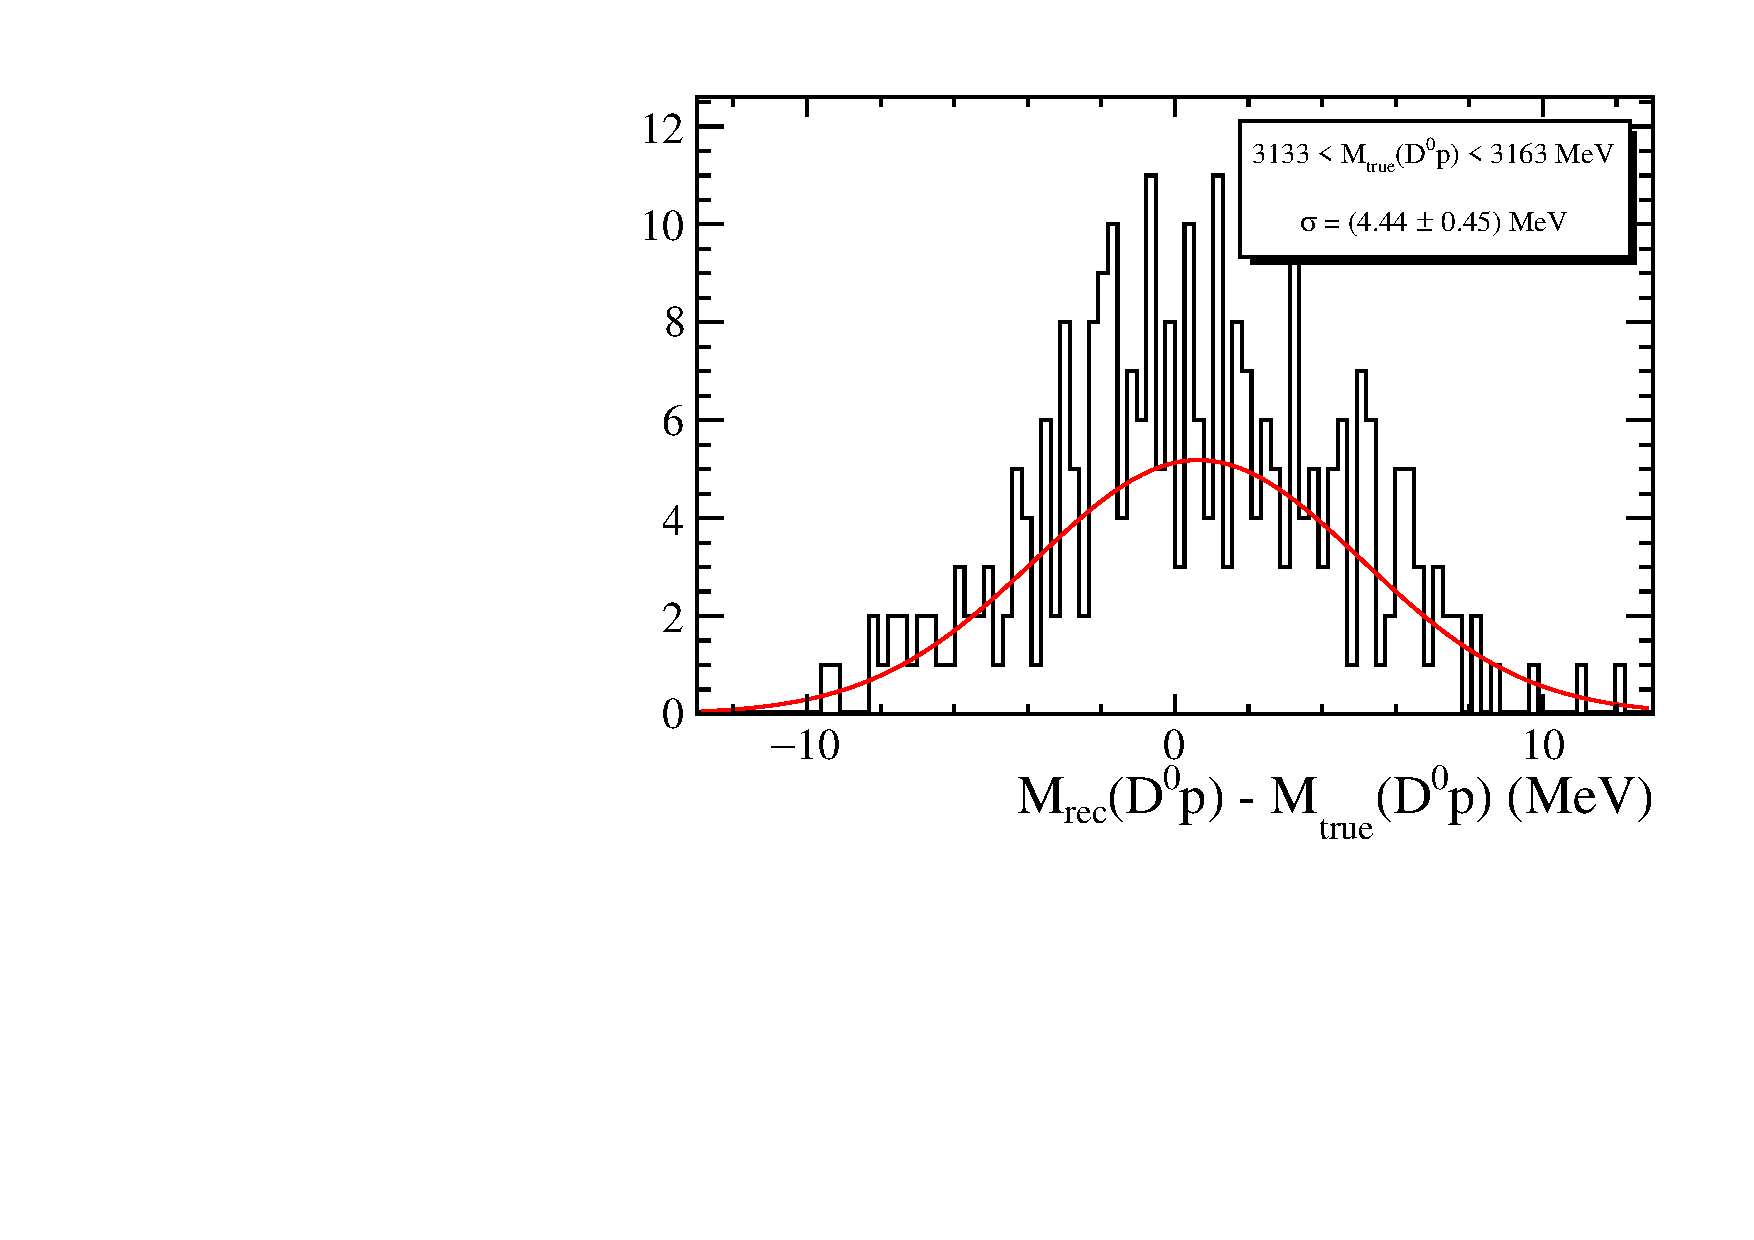
\includegraphics[width=0.32\textwidth]{LbToD0p/massresolution/massresolution_011} \\
	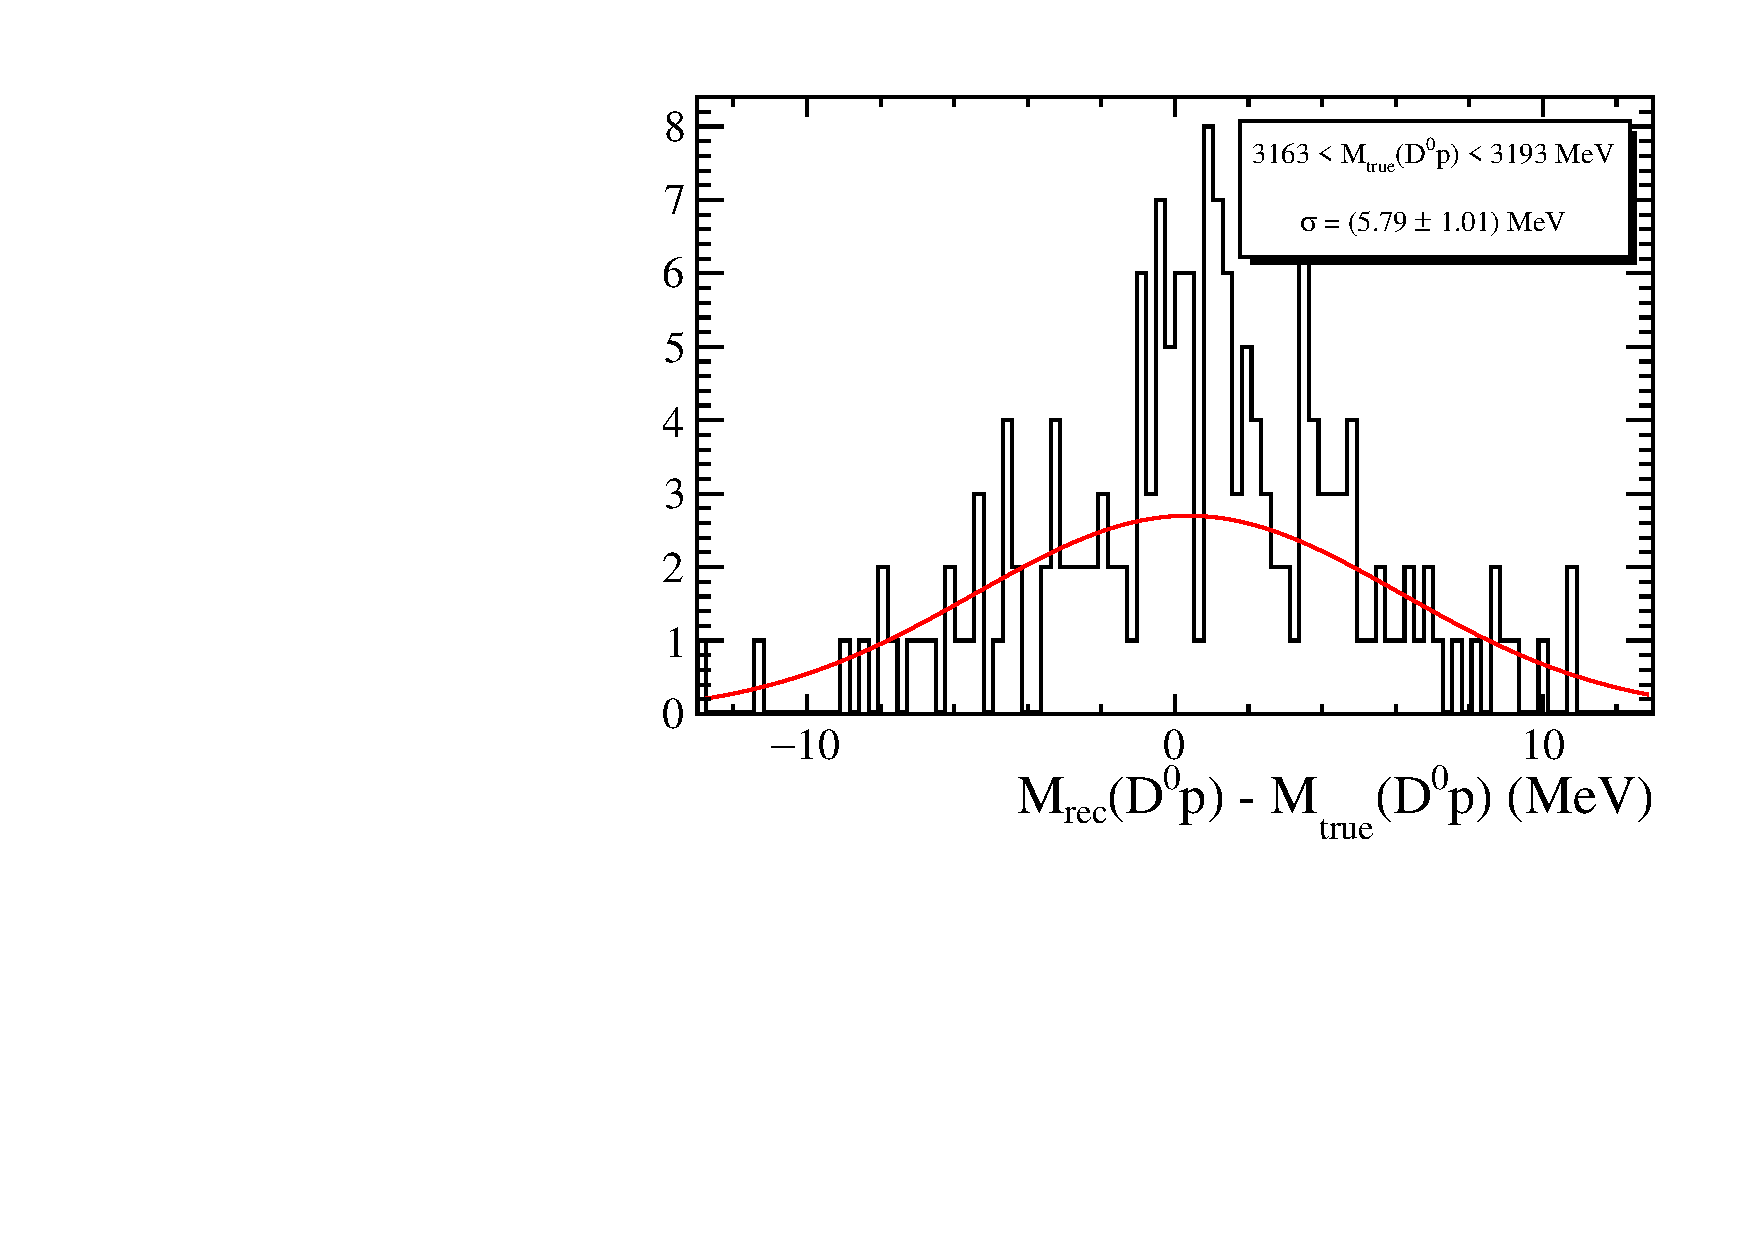
\includegraphics[width=0.32\textwidth]{LbToD0p/massresolution/massresolution_012}
	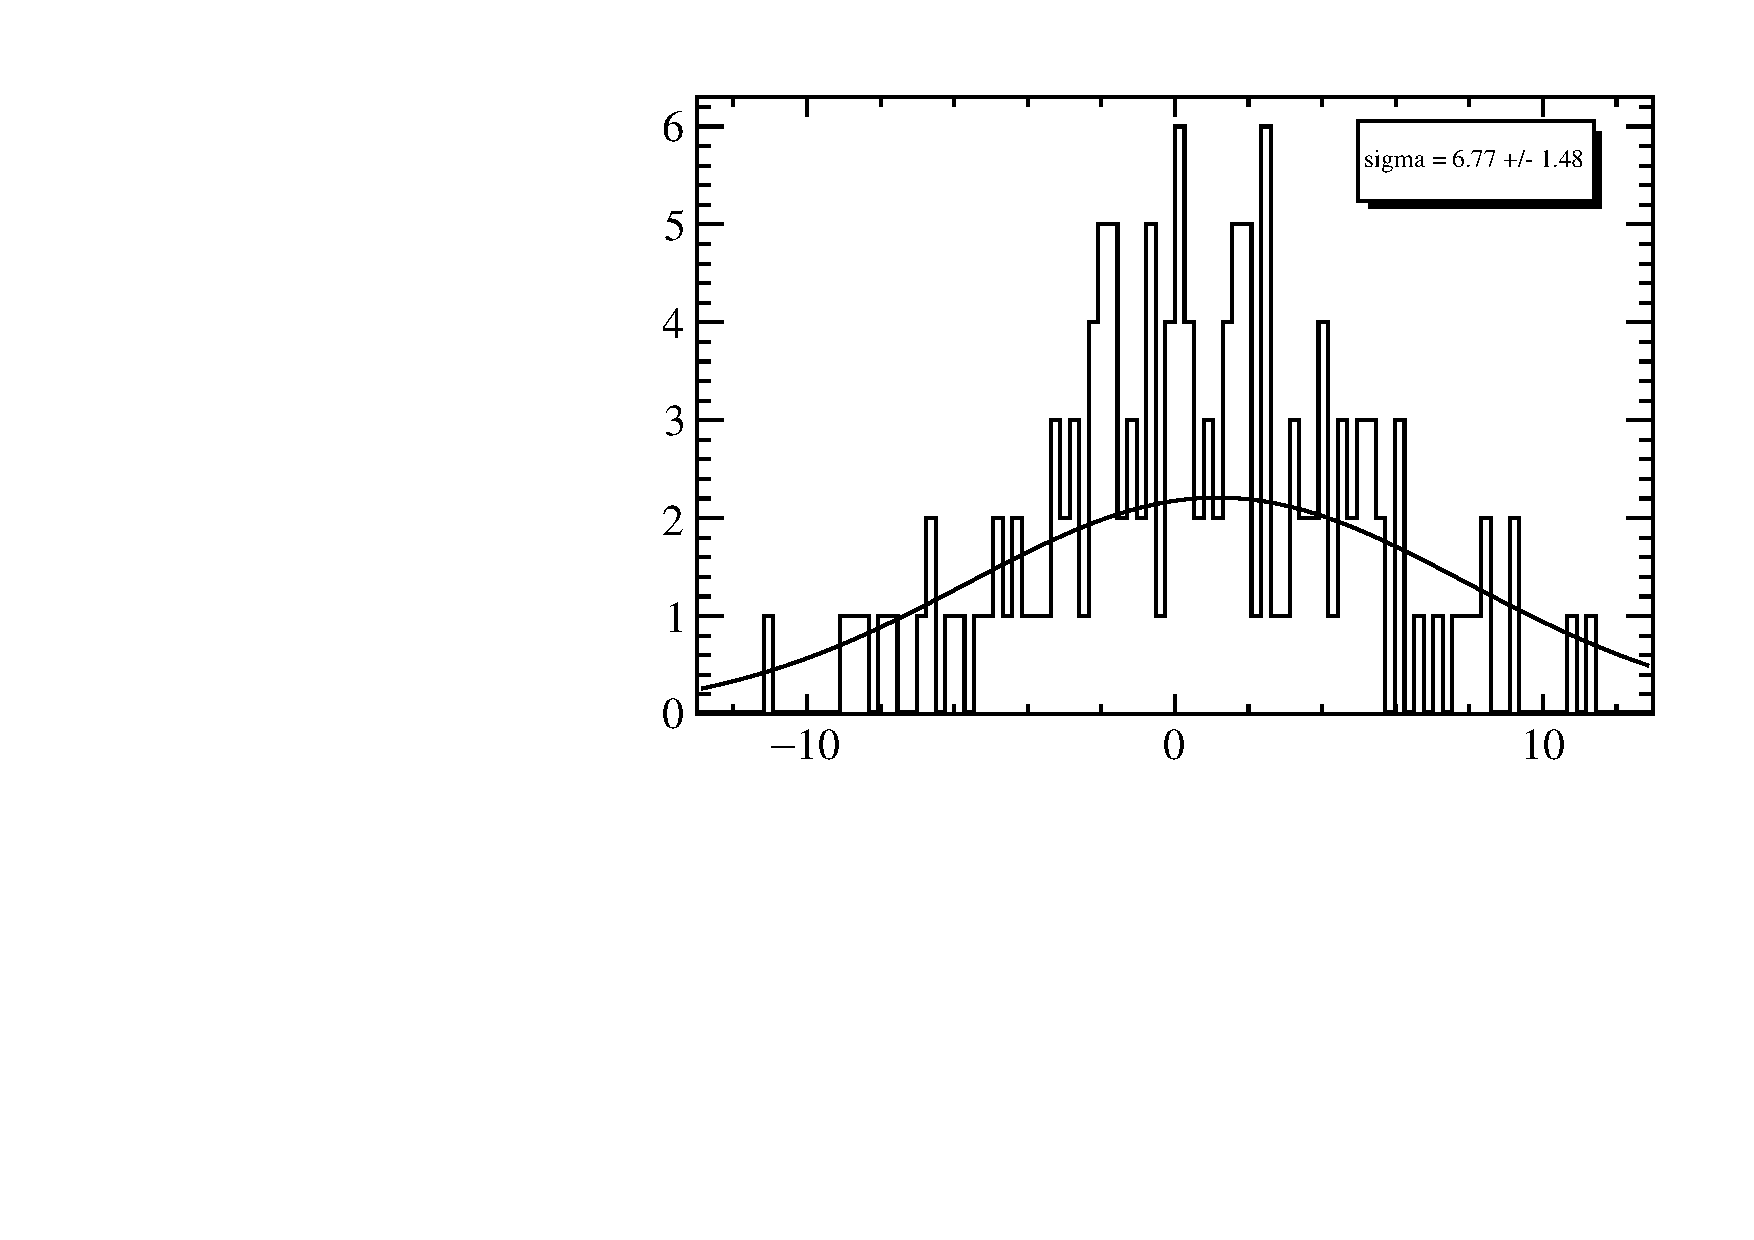
\includegraphics[width=0.32\textwidth]{LbToD0p/massresolution/massresolution_013}
	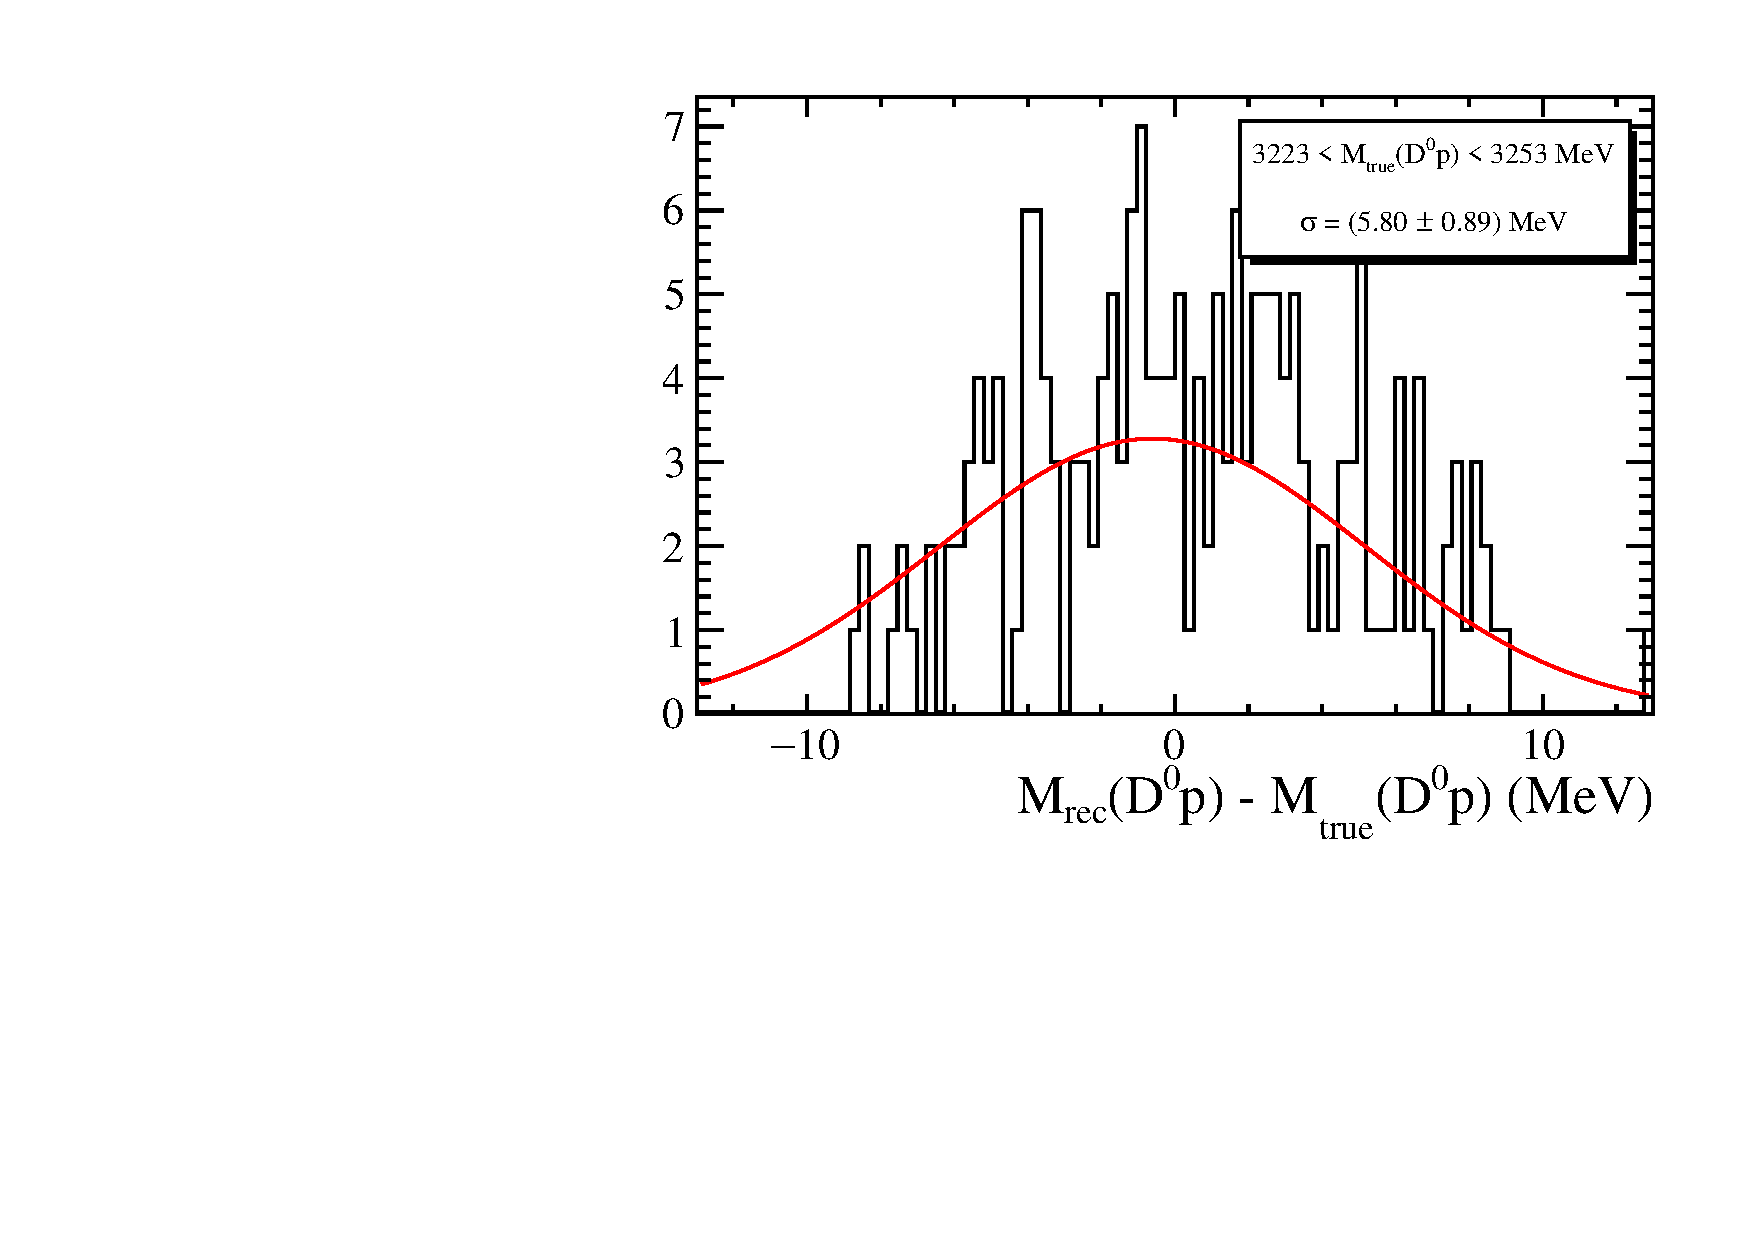
\includegraphics[width=0.32\textwidth]{LbToD0p/massresolution/massresolution_014} \\
	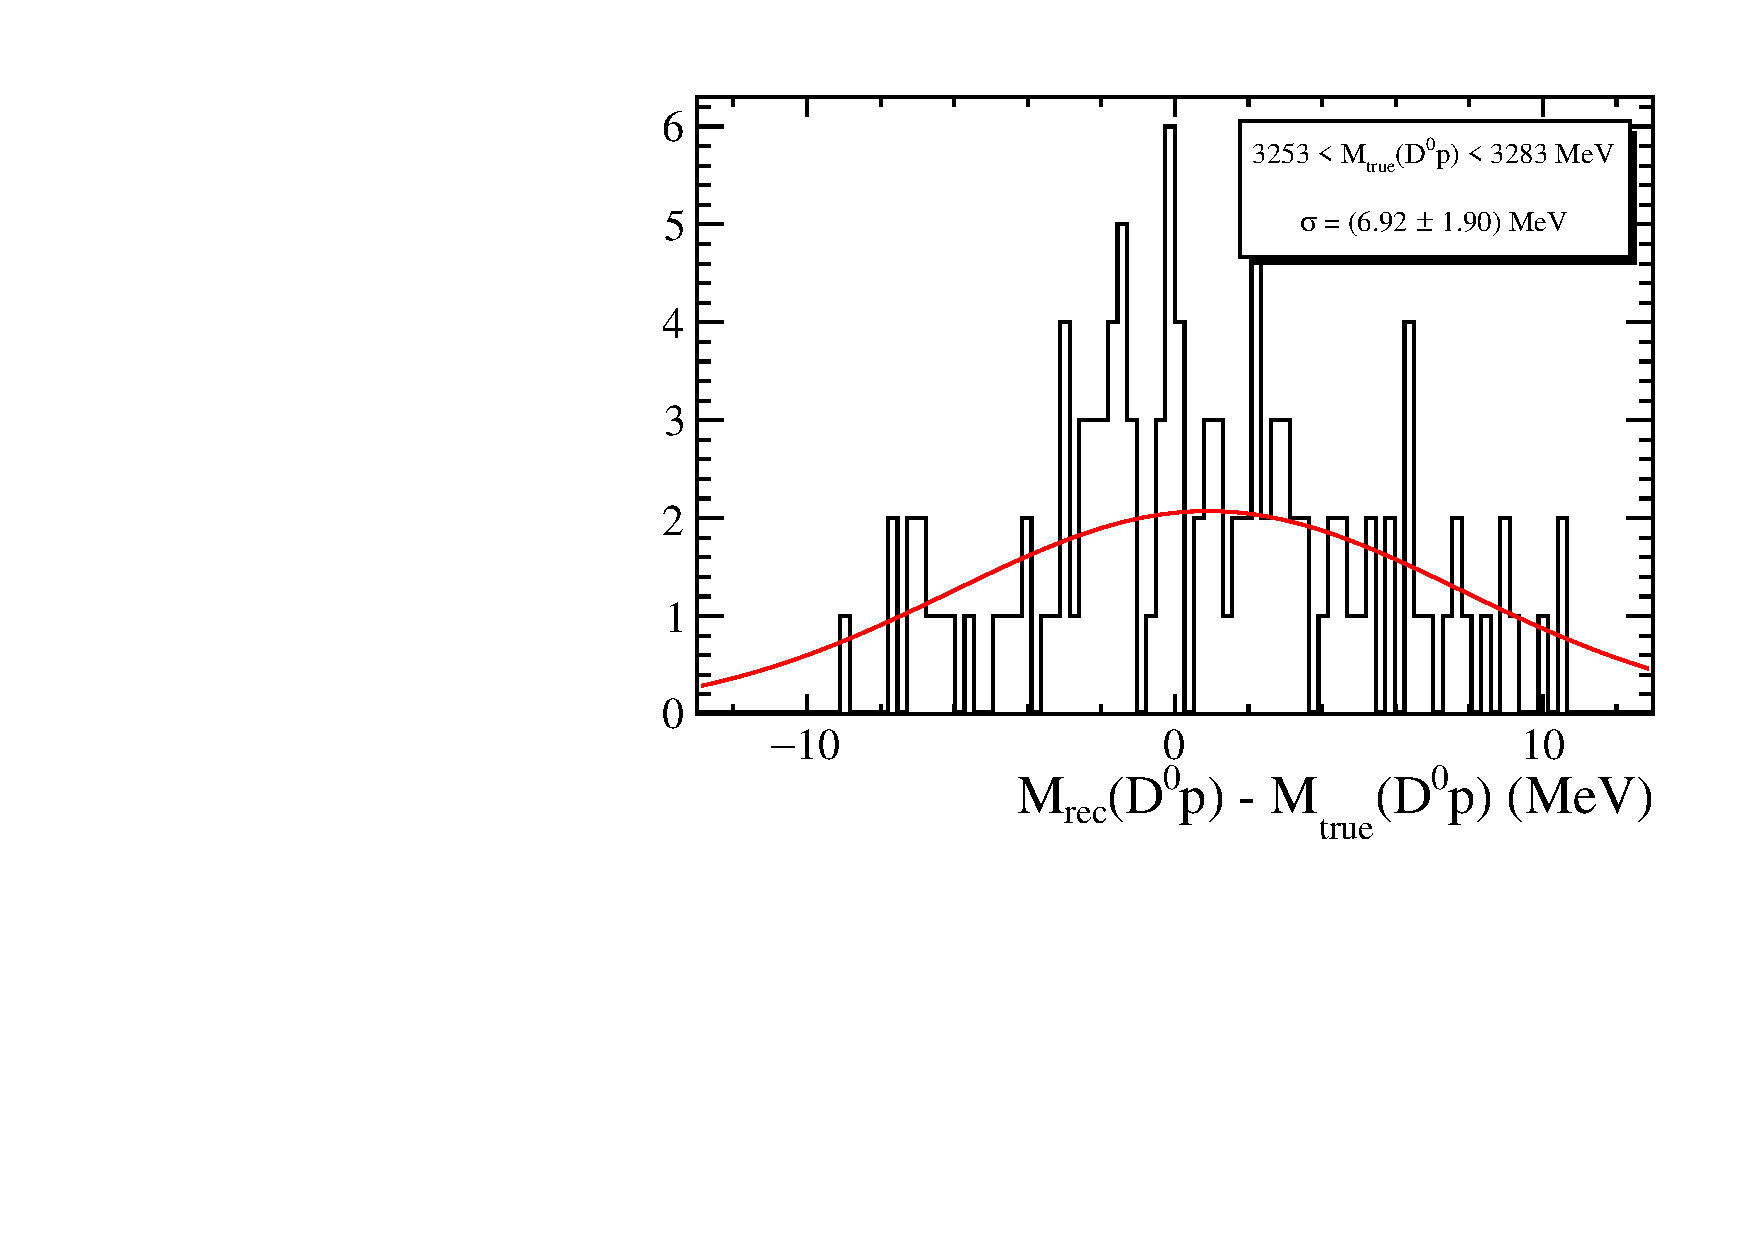
\includegraphics[width=0.32\textwidth]{LbToD0p/massresolution/massresolution_015}
	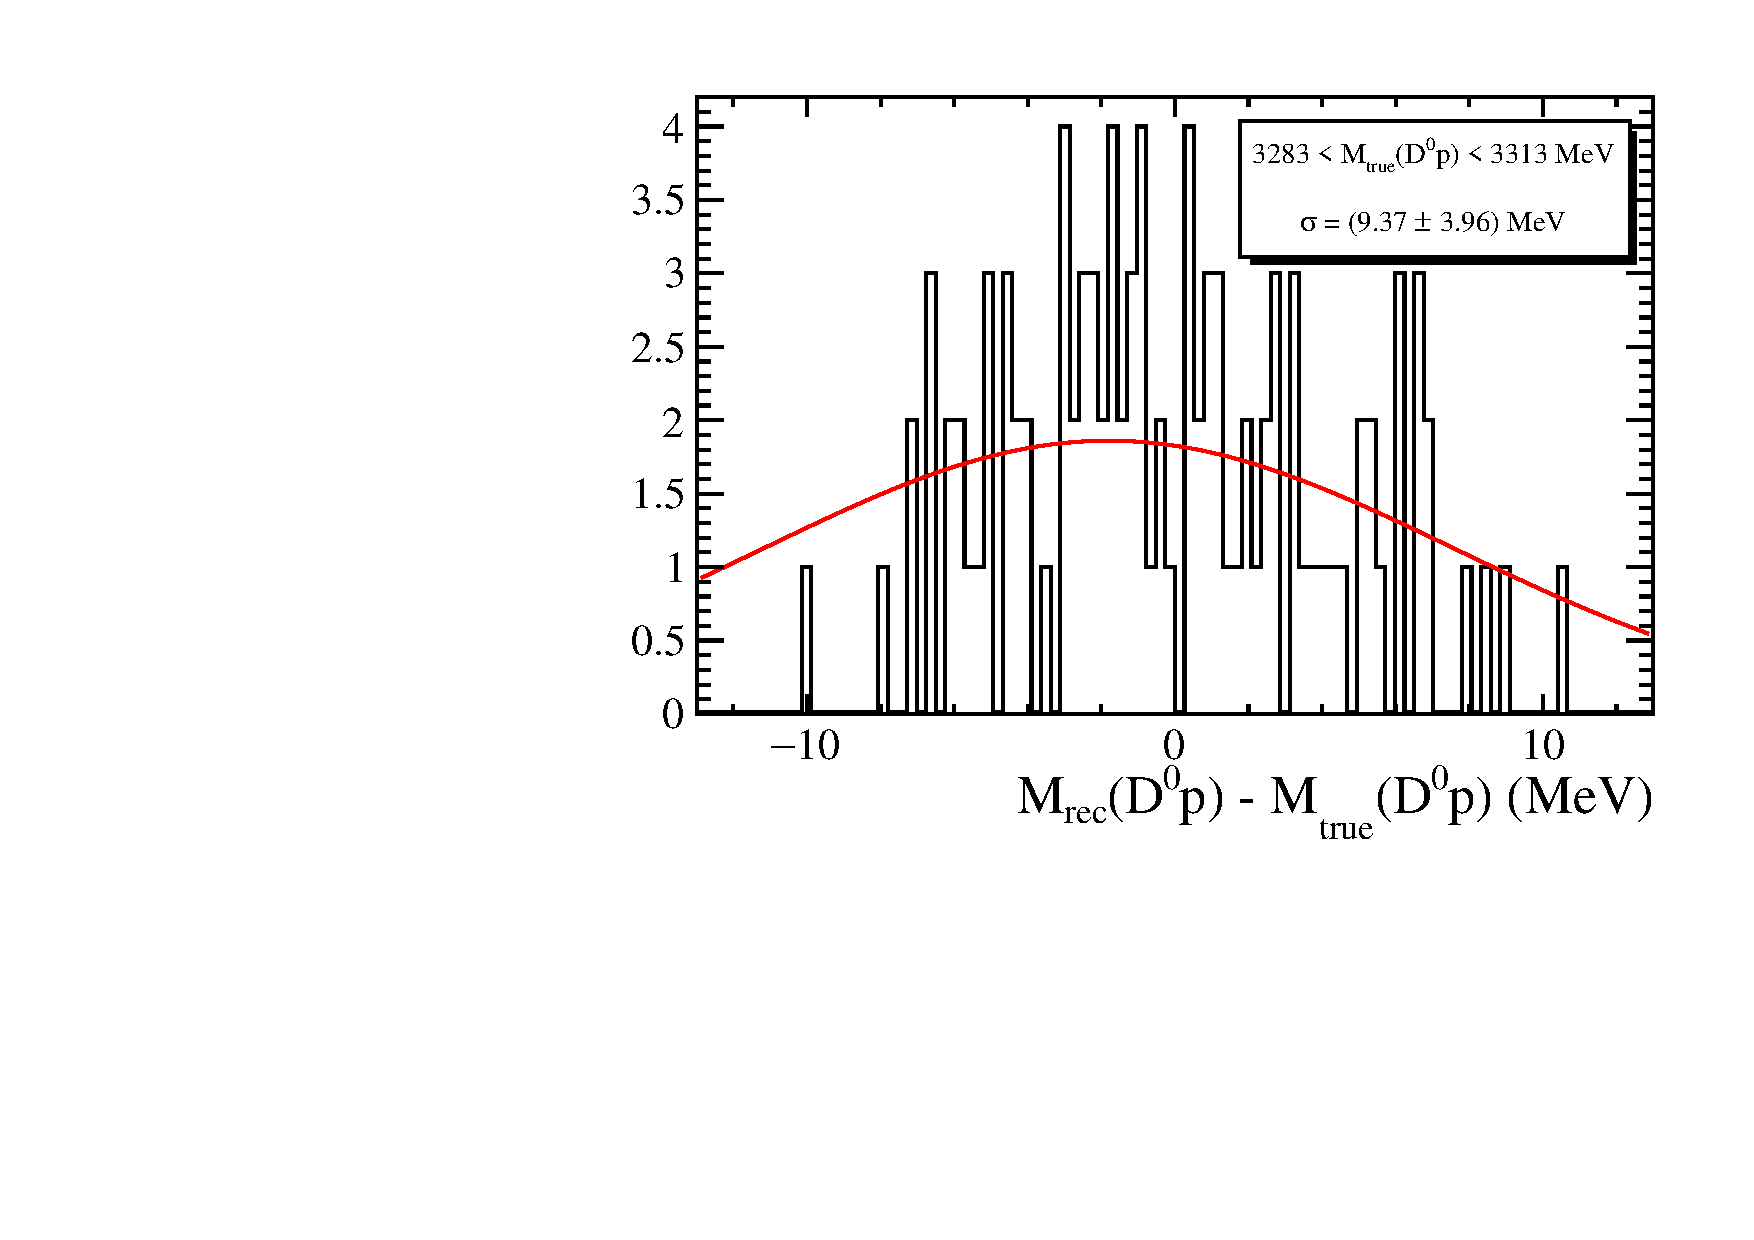
\includegraphics[width=0.32\textwidth]{LbToD0p/massresolution/massresolution_016}
	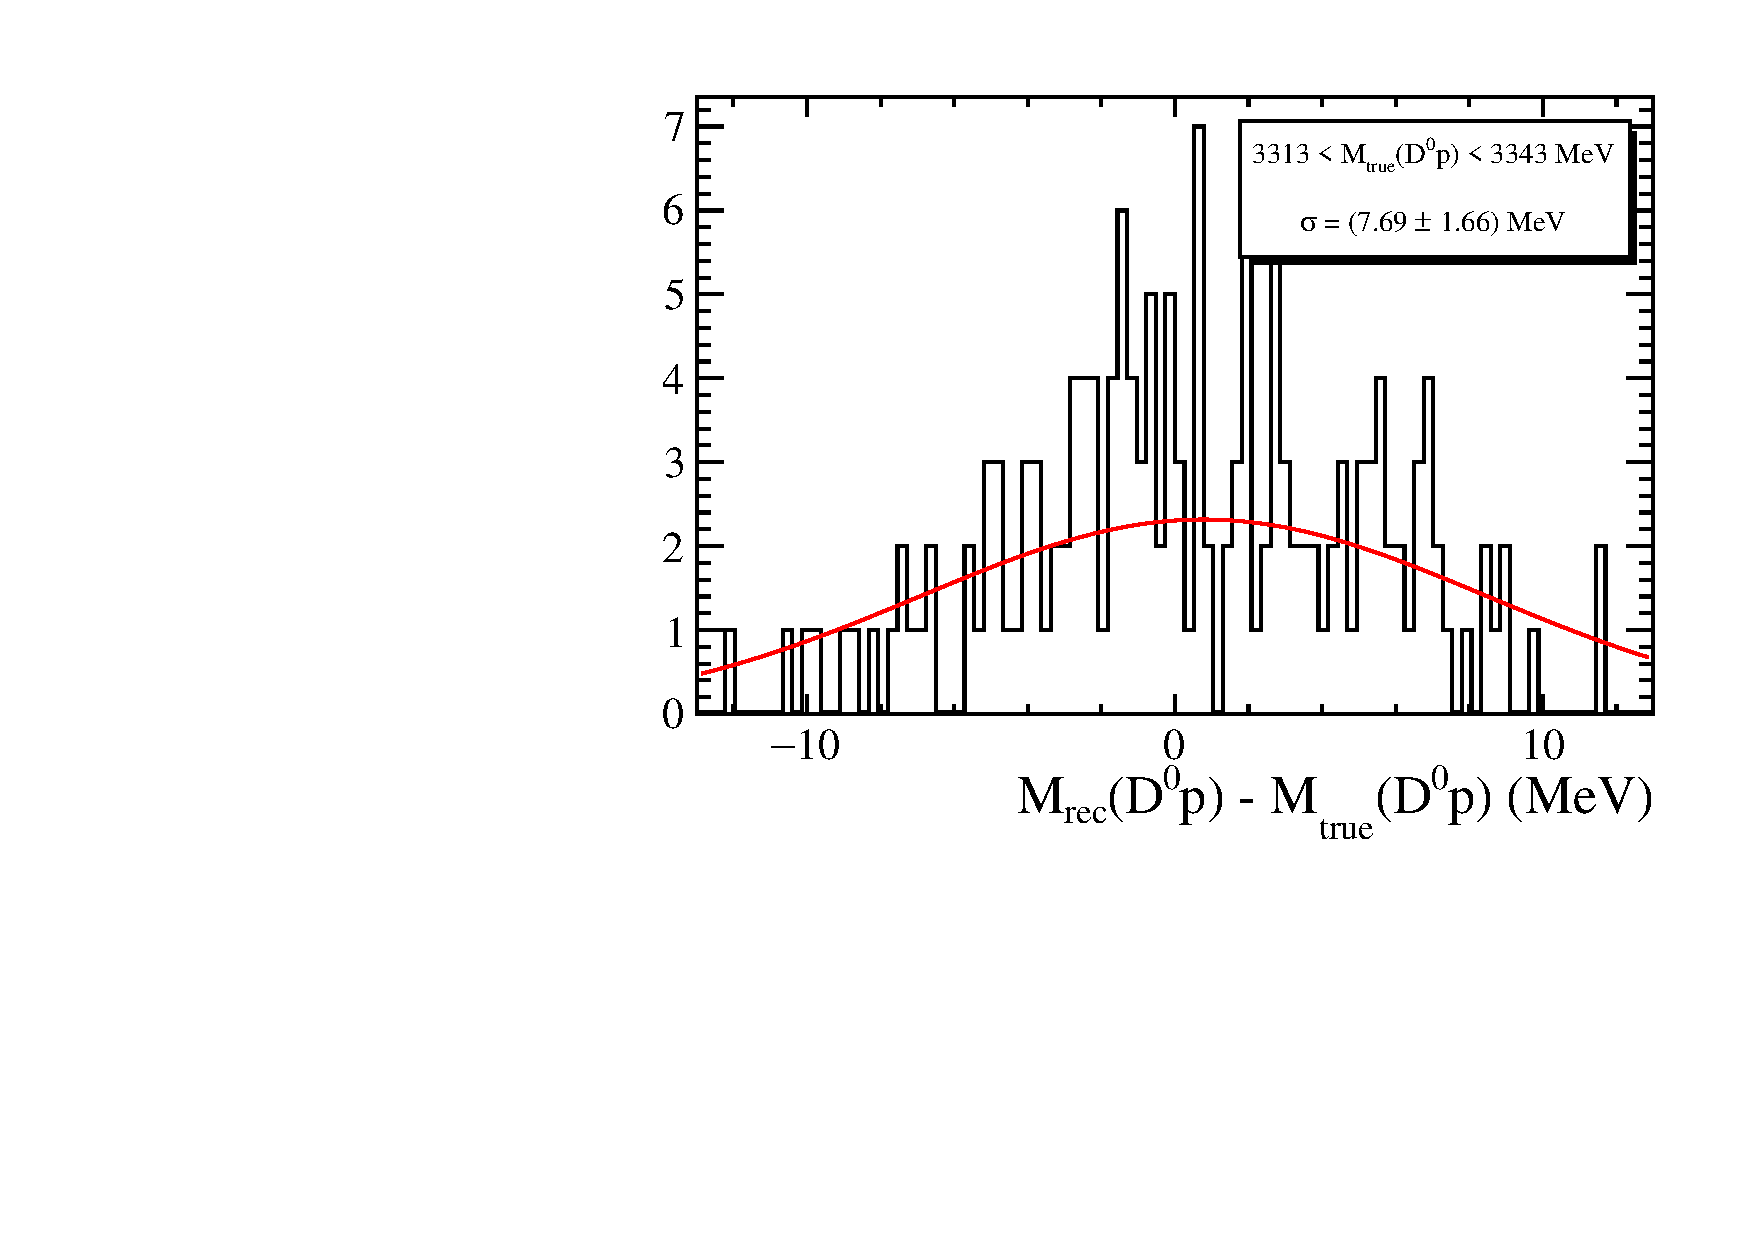
\includegraphics[width=0.32\textwidth]{LbToD0p/massresolution/massresolution_017} \\
	%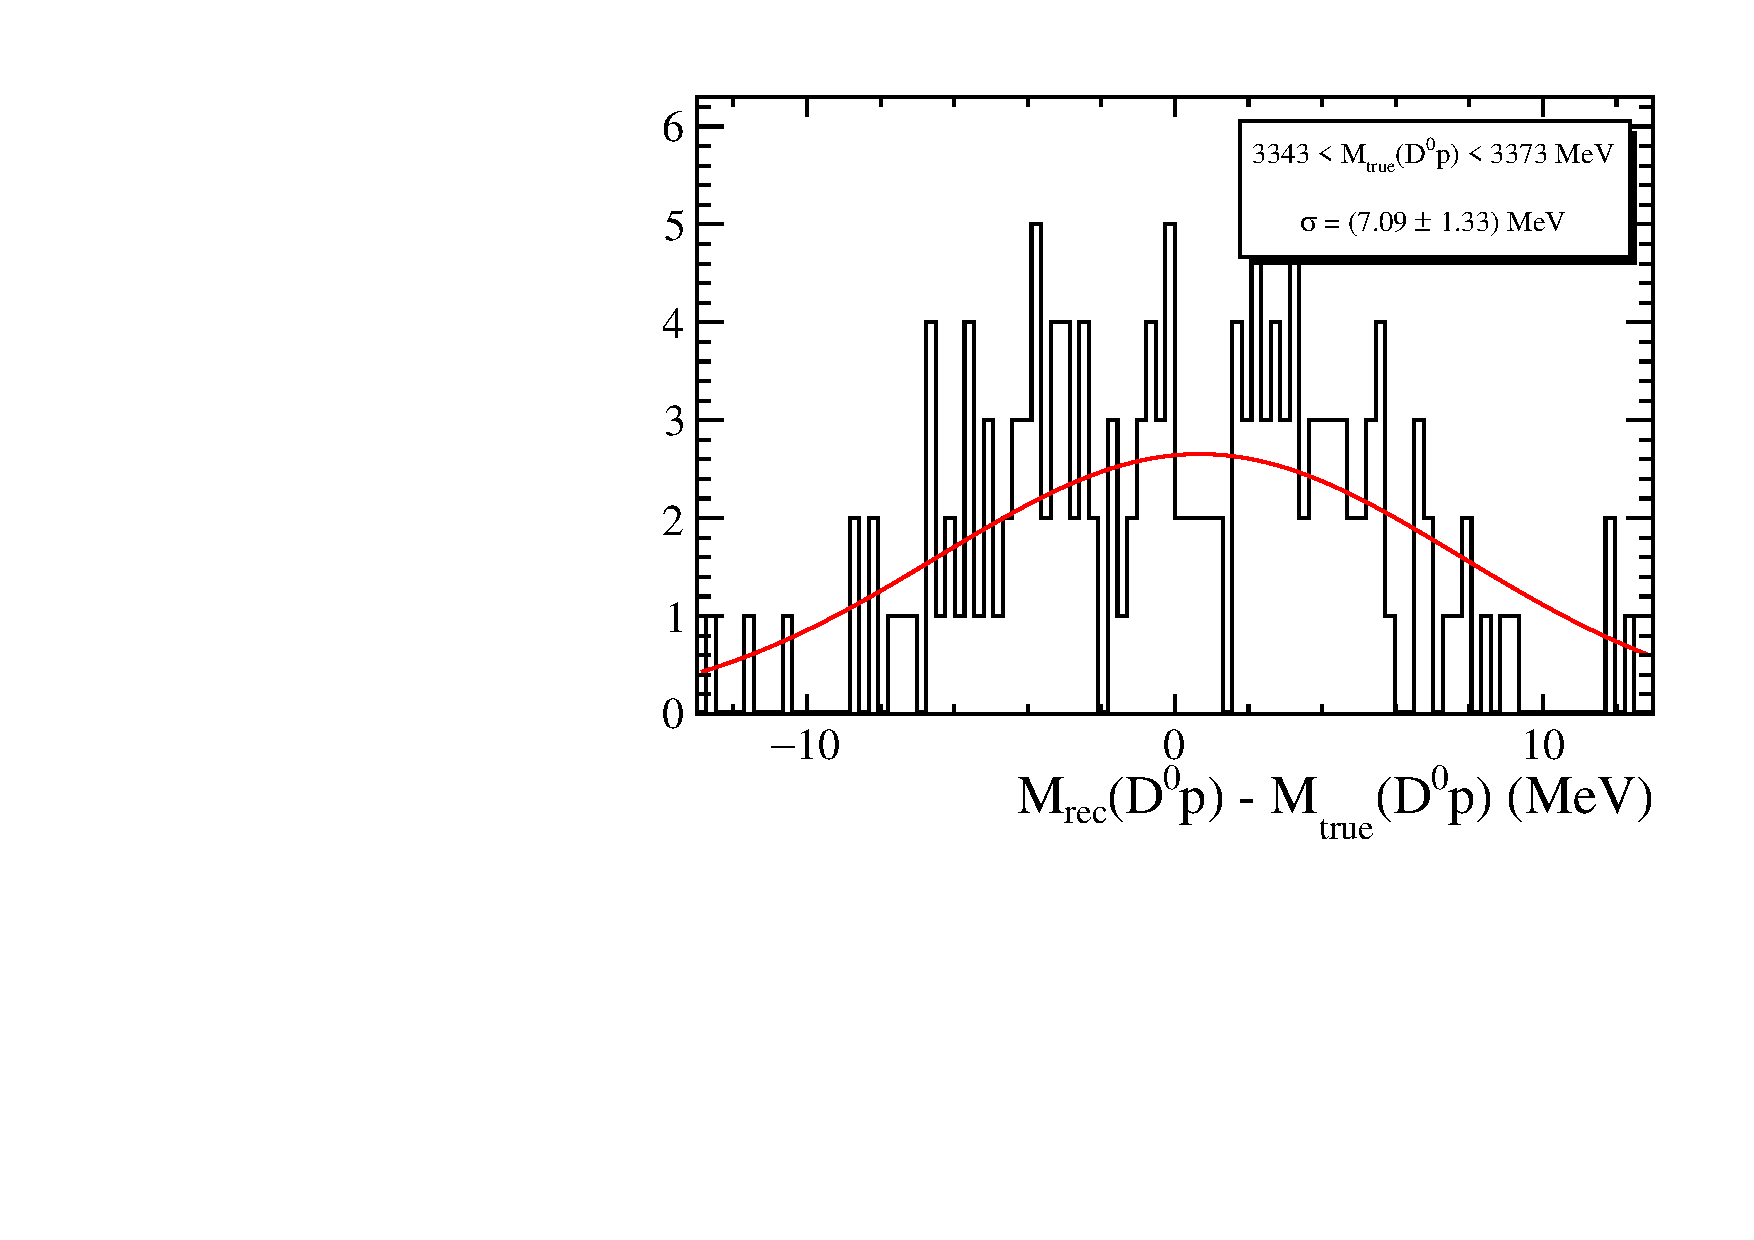
\includegraphics[width=0.32\textwidth]{LbToD0p/massresolution/massresolution_018}
	%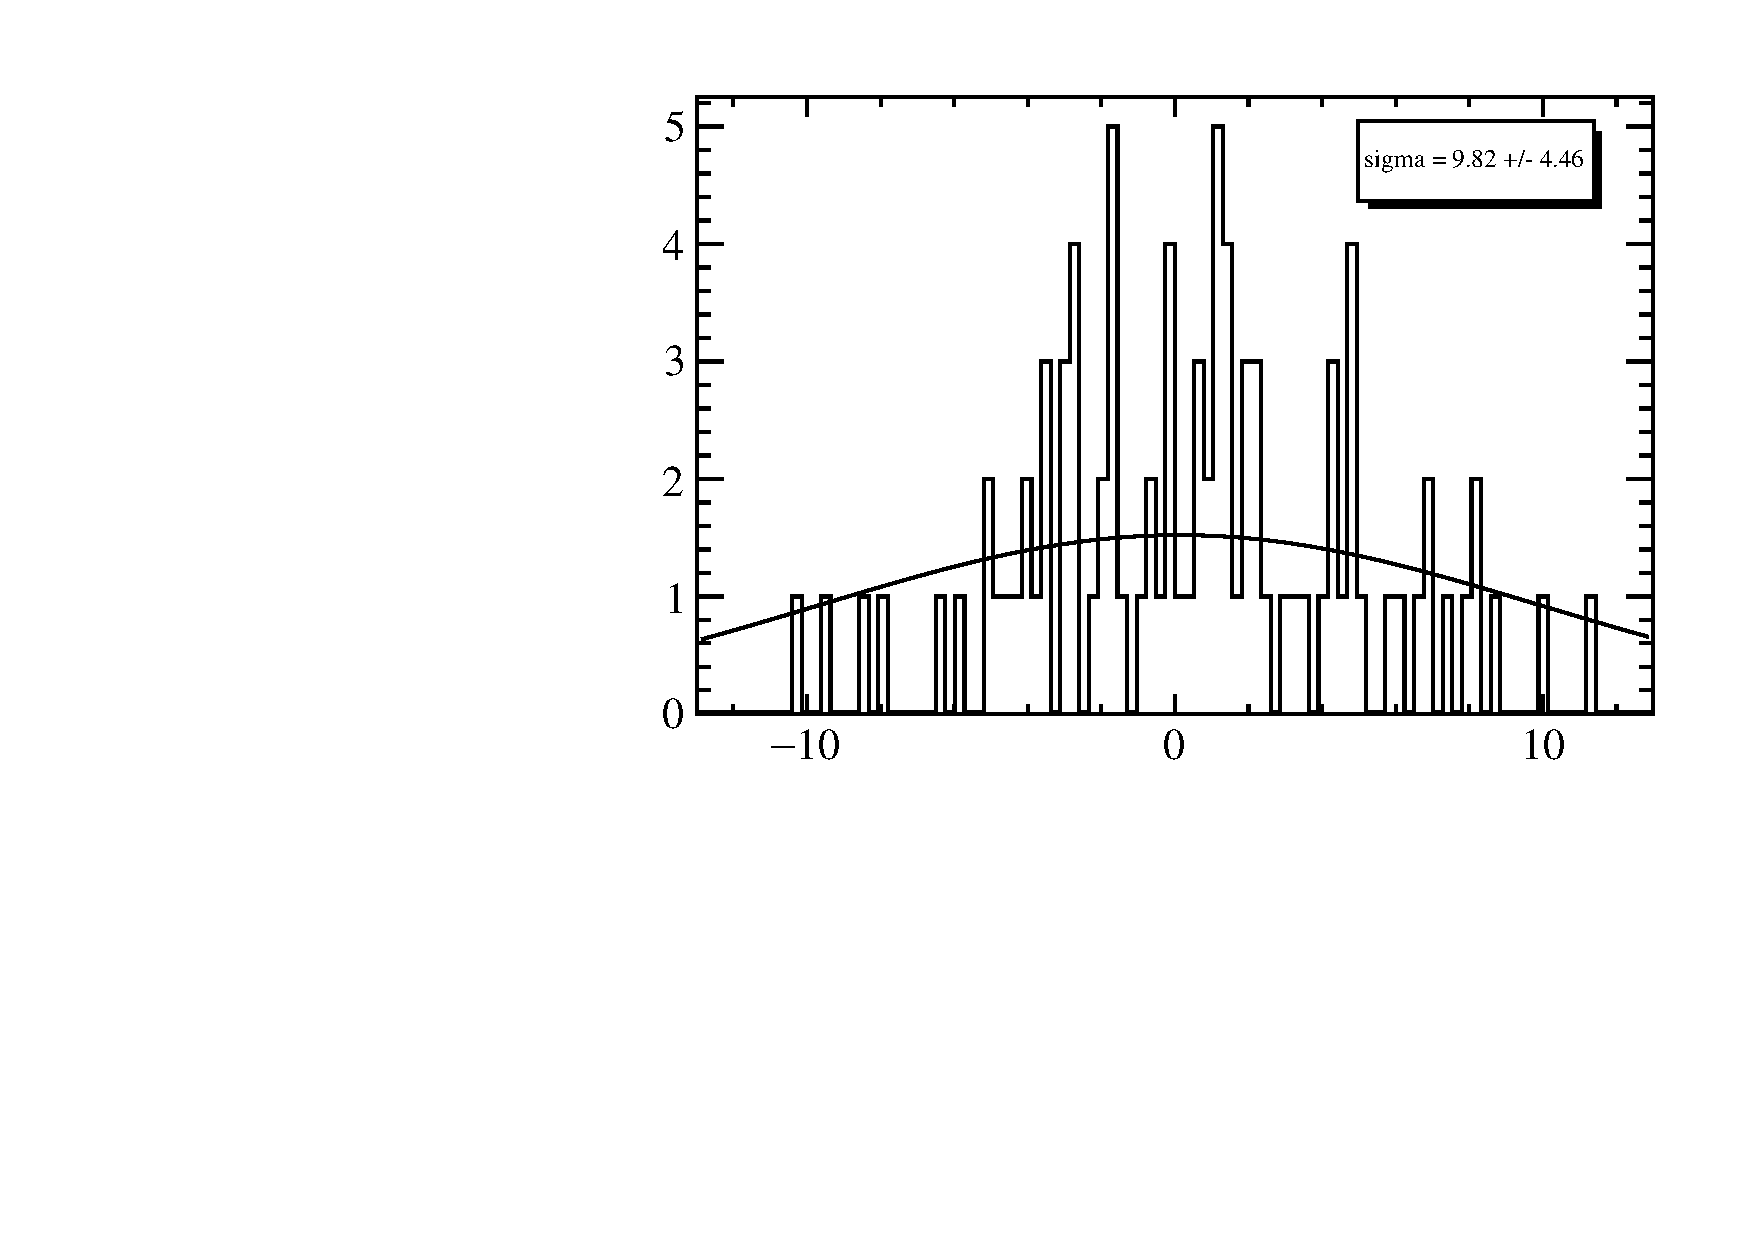
\includegraphics[width=0.32\textwidth]{LbToD0p/massresolution/massresolution_019}
	%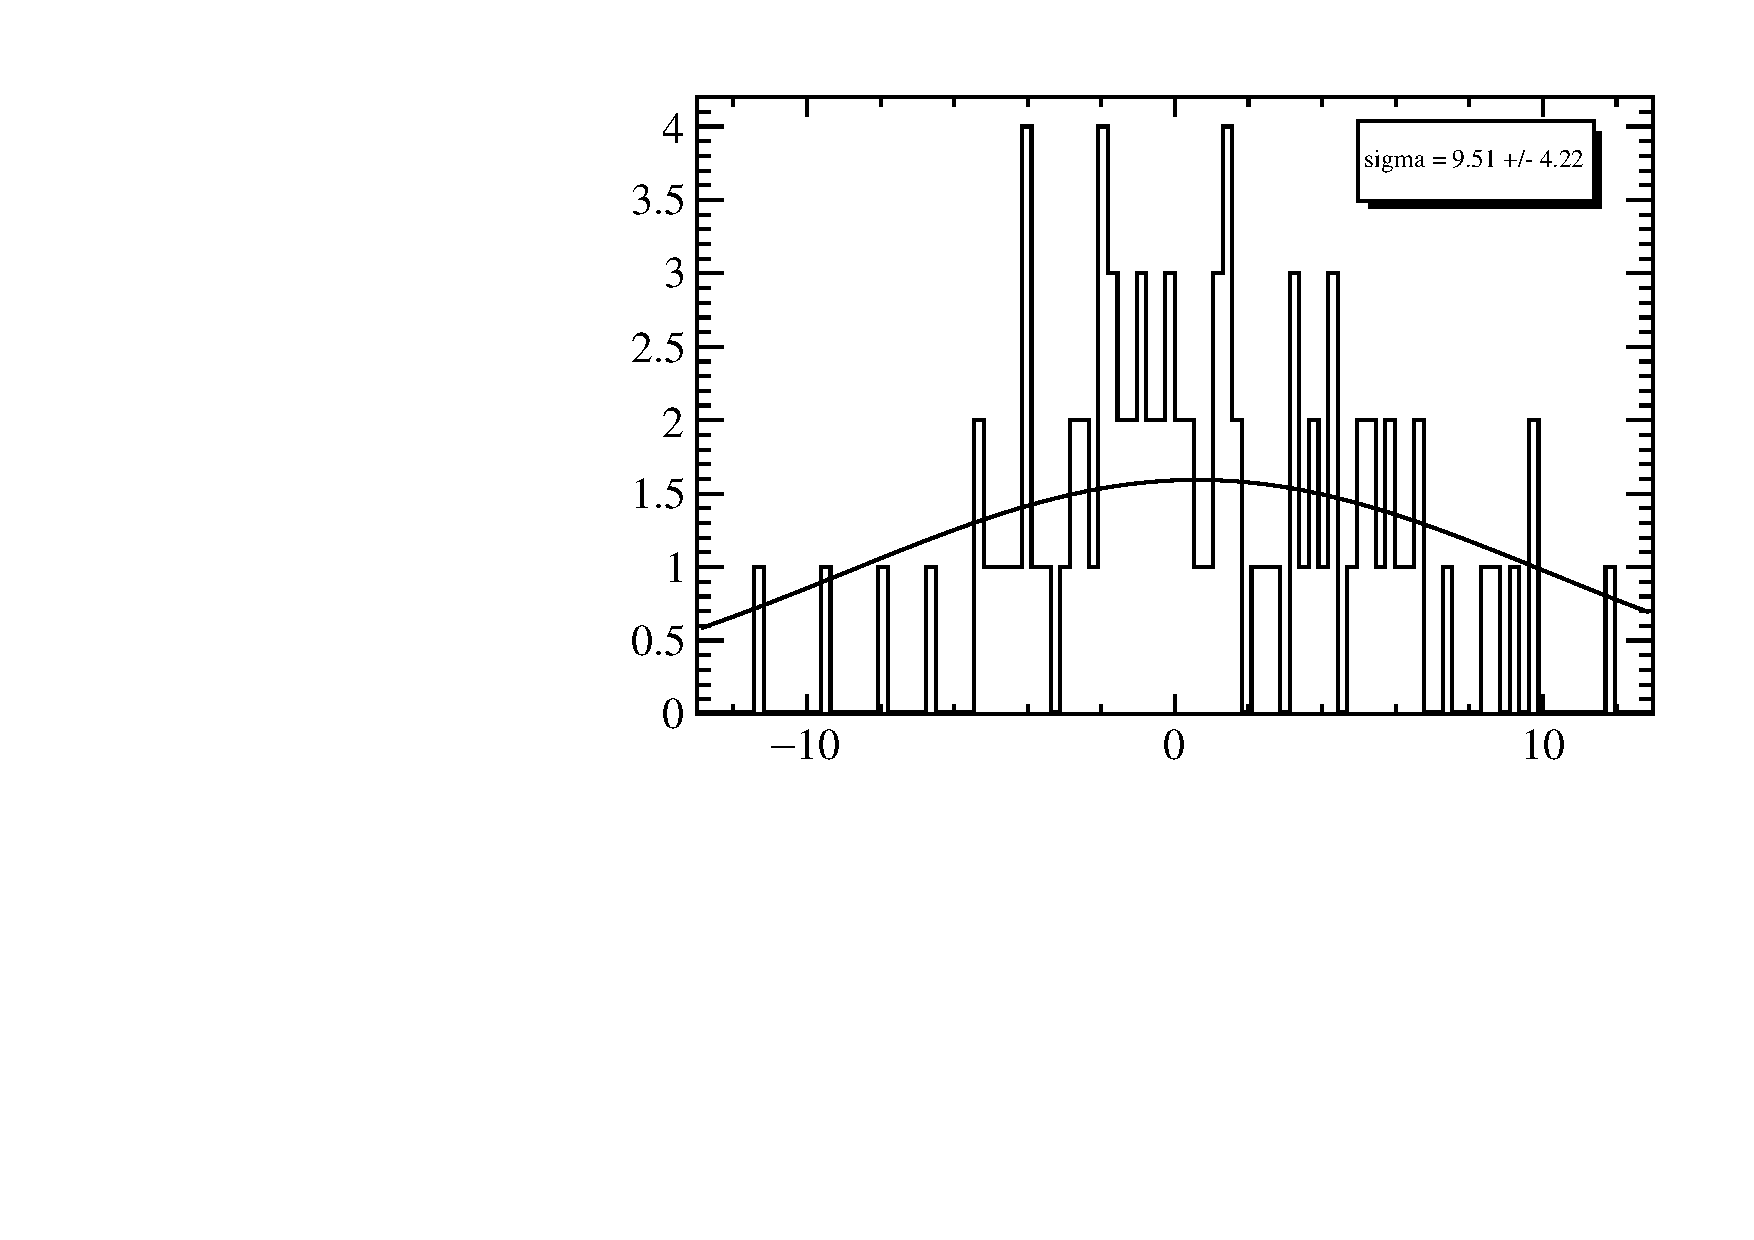
\includegraphics[width=0.32\textwidth]{LbToD0p/massresolution/massresolution_020} \\
	%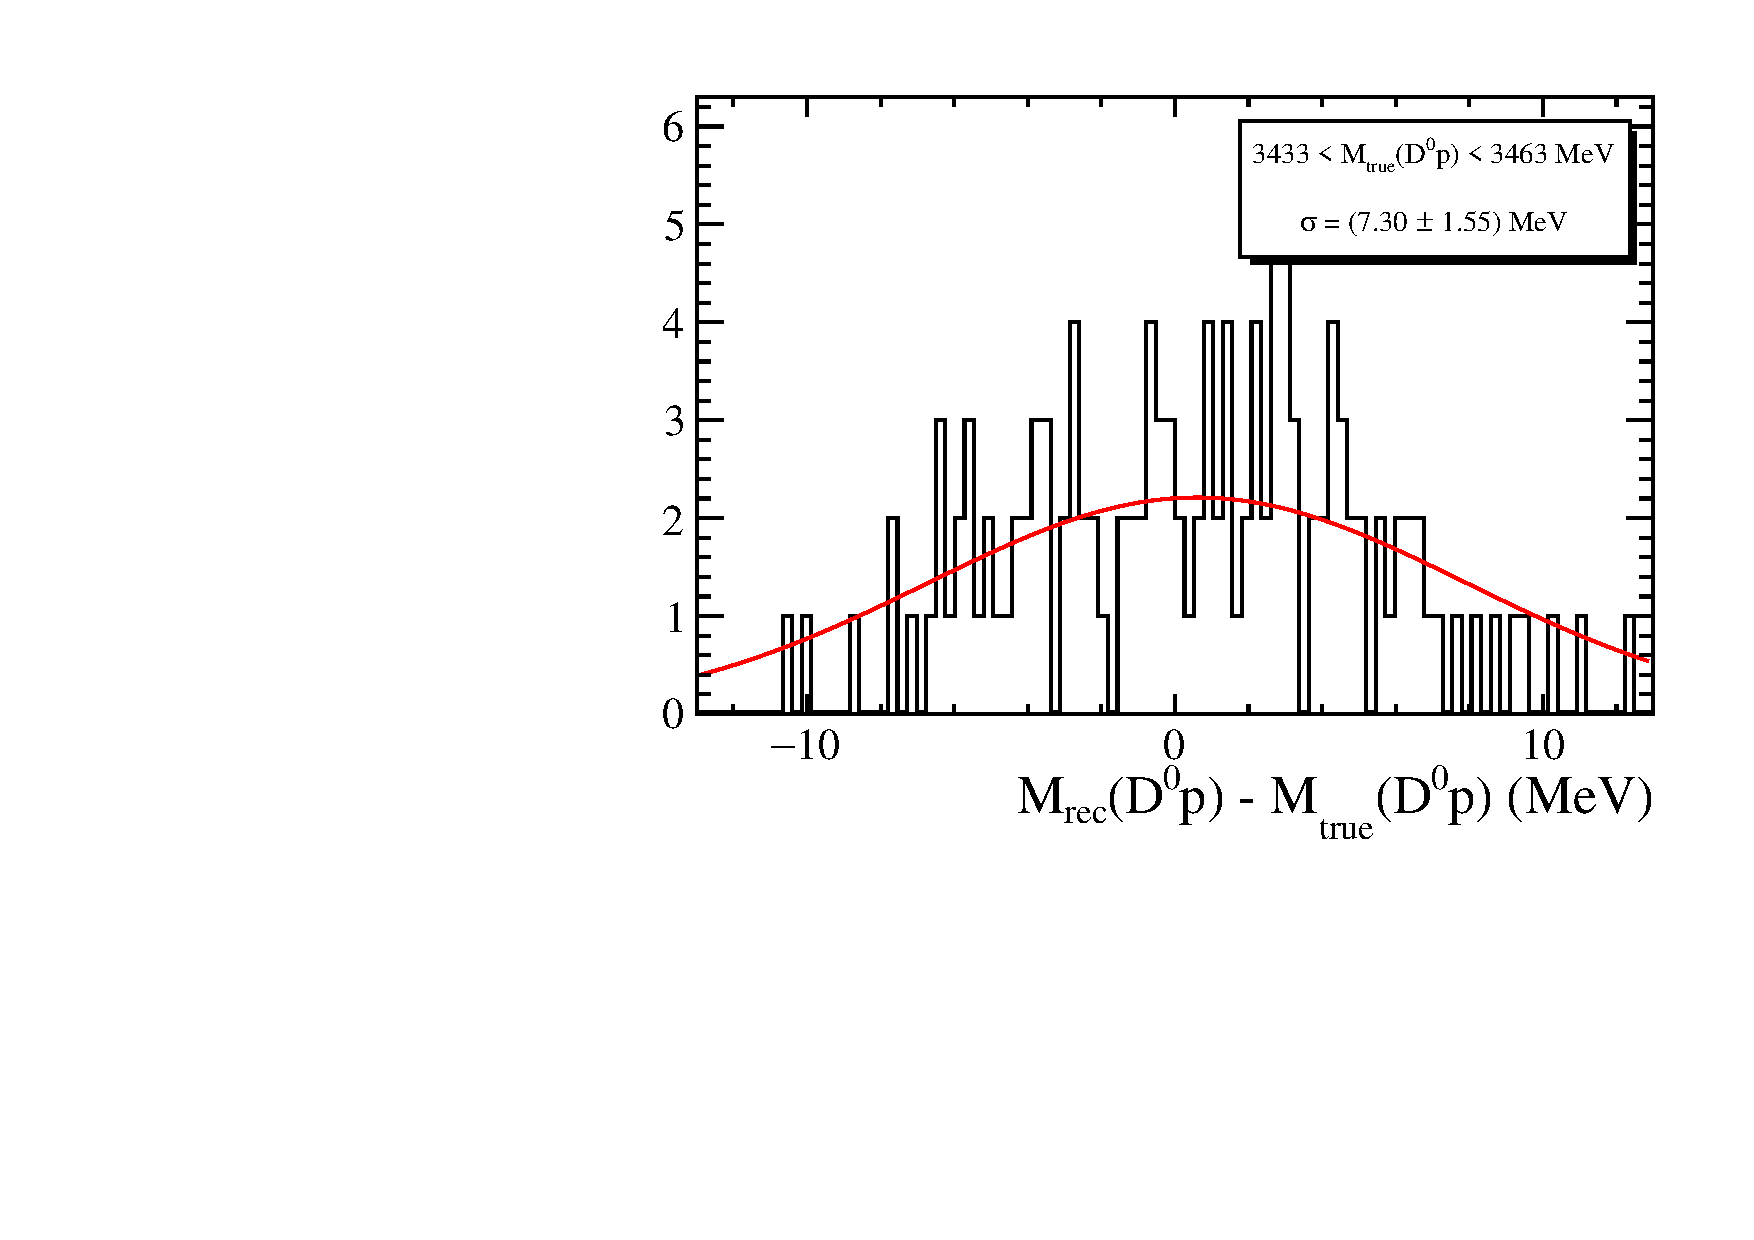
\includegraphics[width=0.32\textwidth]{LbToD0p/massresolution/massresolution_021}
	%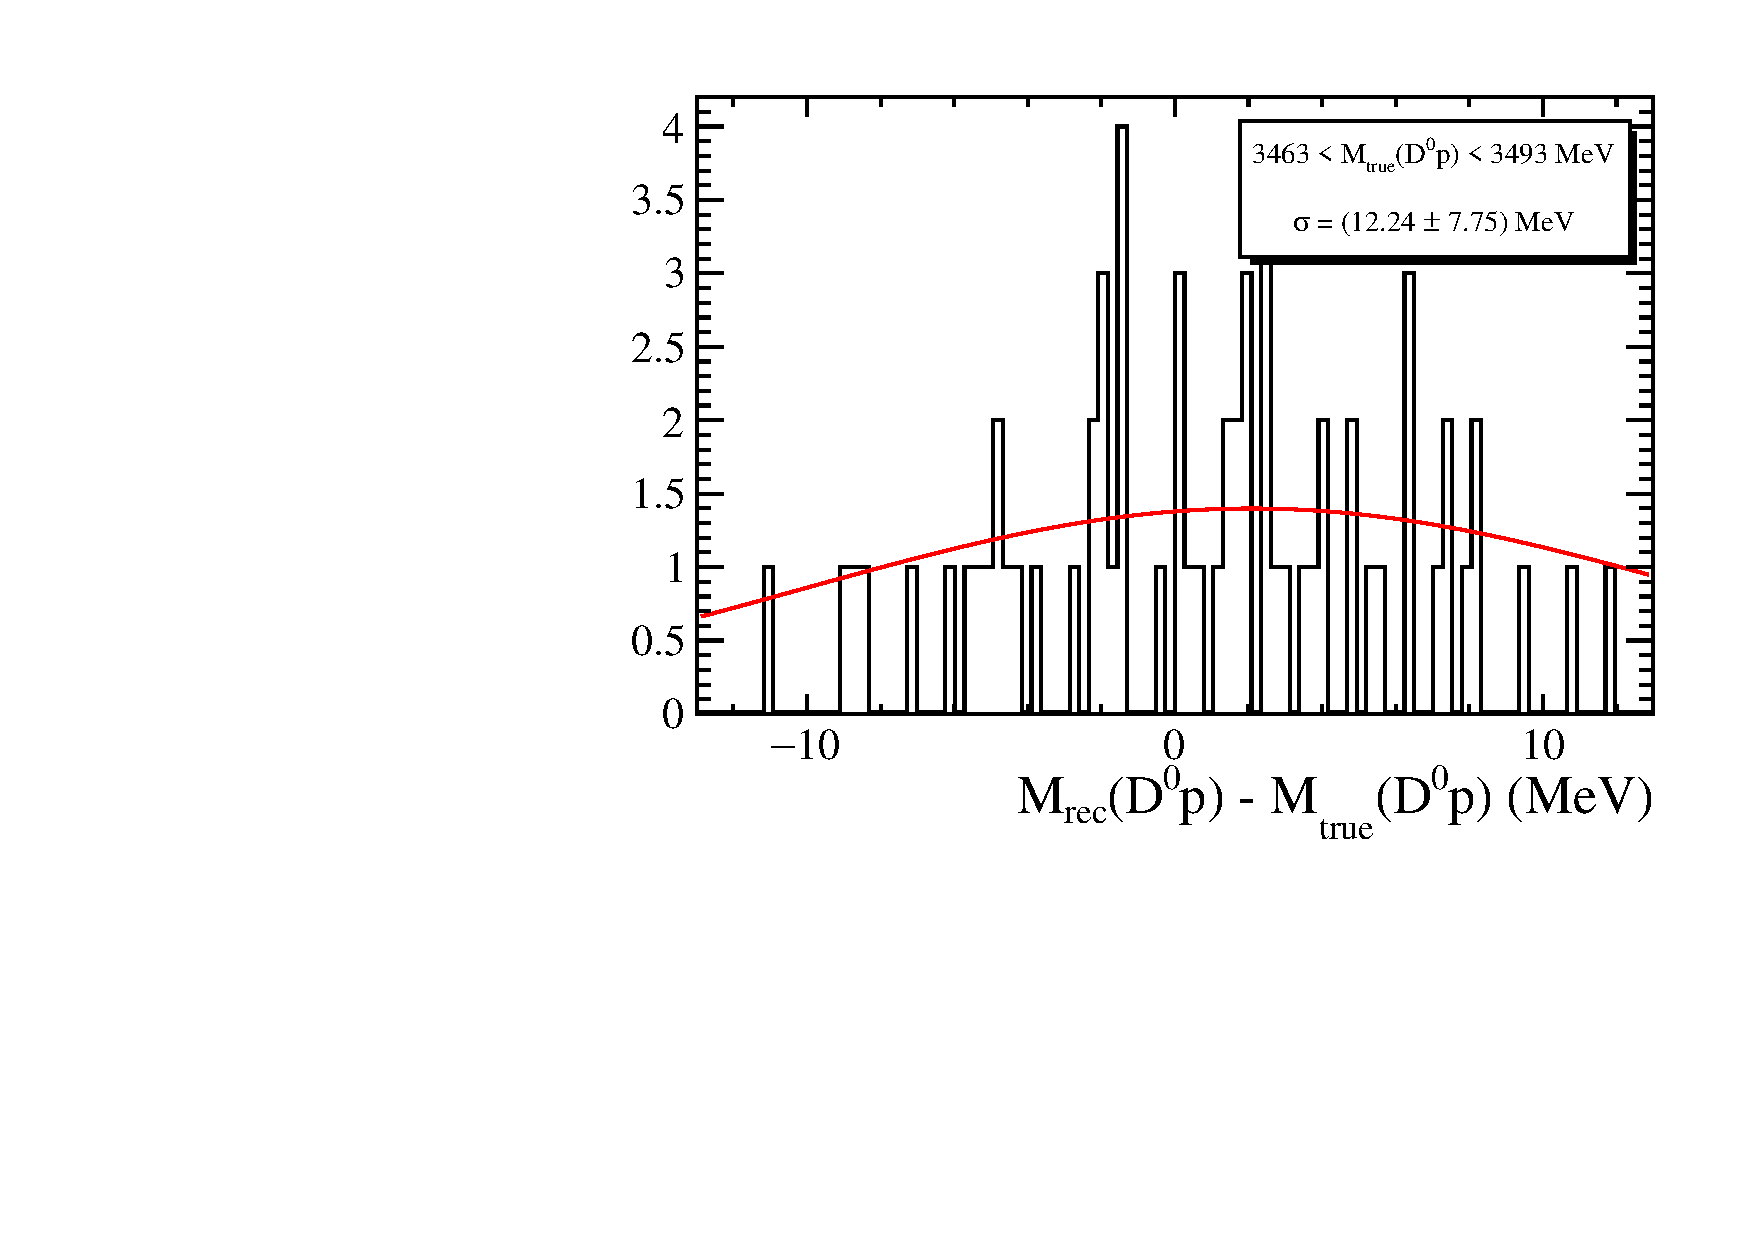
\includegraphics[width=0.32\textwidth]{LbToD0p/massresolution/massresolution_022}
	%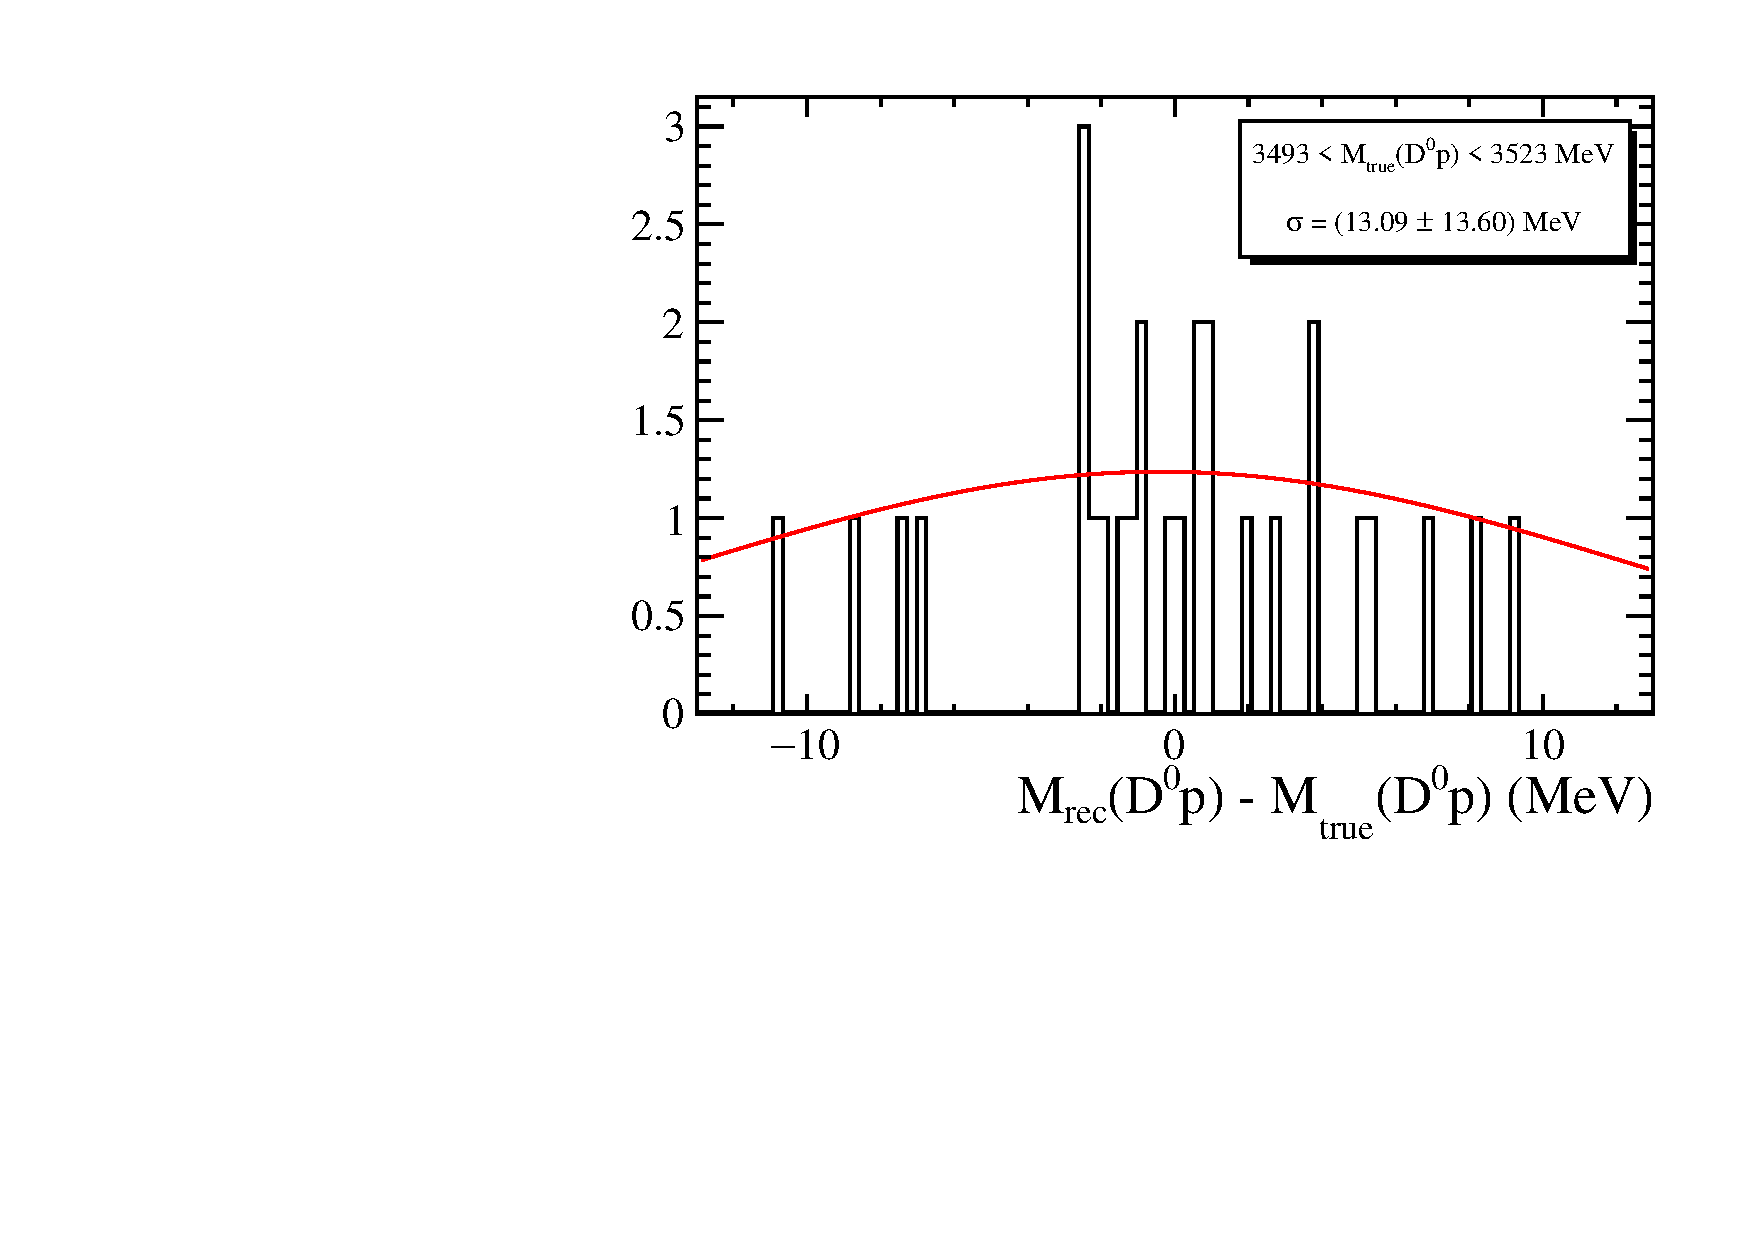
\includegraphics[width=0.32\textwidth]{LbToD0p/massresolution/massresolution_023} \\
	\caption{Fit of a Gaussian to the difference between generated and reconstructed \Dz\proton mass (simulation sample) in bins of 30\mev \Dz\proton) mass (first 18 bins of 24 shown here). The width of the Gaussian is taken as massresolution for the respective bin.}
    \label{fig:massresolution_all}
\end{figure}
